%! Unidad 3 — Estructura atómica y tabla periódica (teoría, ejemplos resueltos, ejercicios por apartados y prácticas)
%! Fuente: Fuentes/Quimica/Unidad 3 (capturas 502-515 y solucionario). Texto reescrito; datos de los ejercicios cambiados y recalculados.
%! Constantes: h = 6,626·10^-34 J·s; c = 3,00·10^8 m/s; N_A = 6,022·10^23 mol^-1; R_H = 1,097·10^7 m^-1;
%!             E_n = -2,18·10^-18 J / n^2 = -13,6 eV / n^2; 1 eV = 1,602·10^-19 J.
%! Macros del principal: \conf{1s^2\,2s^2} (configuraciones electrónicas) y \orbcaja{\uparrow\downarrow} (diagramas de orbitales).
%! Convención para el electrón diferenciador: los orbitales se llenan de m = -l a m = +l, primero con s = +1/2.

\section*{Para empezar: ¿qué hay dentro de un átomo?}
\addcontentsline{toc}{section}{Para empezar: ¿qué hay dentro de un átomo?}

Las propiedades de toda la materia (su color, si conduce la electricidad, si reacciona con el oxígeno o si es un gas a
temperatura ambiente) dependen de cómo son por dentro los átomos que la forman. Por eso, desde hace más de dos siglos, la
ciencia intenta averiguar cómo es un átomo. Ha sido un camino lleno de propuestas, errores, predicciones acertadas y aciertos
parciales, recorrido por decenas de científicas y científicos, que ha llevado hasta el modelo actual.

Ese conocimiento tiene muchísimas aplicaciones: el \textbf{láser} de los lectores de códigos de barras y de los bisturís, los
\textbf{espectroscopios} que detectan cantidades minúsculas de contaminantes en el aire o de sustancias dopantes en la sangre,
los fuegos artificiales o las pantallas de nuestros móviles. En esta unidad recorreremos la historia de los modelos atómicos,
aprenderemos a describir dónde están los electrones de un átomo y veremos por qué la tabla periódica tiene la forma que tiene.

%========================================================================================
\section{Recuerda de la ESO}\label{sec:ud3-eso}
%========================================================================================

\paragraph{Ondas.} Una \textbf{onda} transporta \textbf{energía} de un punto a otro sin que haya transporte de materia: el
sonido, las ondas de una cuerda o los círculos que se forman en el agua al tirar una piedra. Una onda se caracteriza por su
\textbf{amplitud}, su \textbf{longitud de onda} y su \textbf{frecuencia}.

\paragraph{Estructura del átomo.} El \textbf{átomo} es la unidad más pequeña de un \textbf{elemento}. En él se distinguen el
\textbf{núcleo}, donde están los \textbf{protones} (carga positiva) y los \textbf{neutrones} (sin carga), y la
\textbf{corteza}, donde se mueven los \textbf{electrones} (carga negativa). Al protón se le asigna carga \(+1\) y al electrón,
\(-1\). Todos los átomos de un mismo elemento tienen el mismo número de protones, que se llama \textbf{número atómico}, \(Z\).
Cada elemento se representa con un \textbf{símbolo} de una o dos letras (la primera en mayúscula).

\paragraph{Átomos e iones.} Un átomo \textbf{neutro} tiene tantos electrones como protones. Si gana electrones se convierte en
un \textbf{ion negativo} o \textbf{anión}; si los pierde, en un \textbf{ion positivo} o \textbf{catión}. La carga del ion se
escribe arriba a la derecha del símbolo. Por ejemplo, el flúor (\(Z = 9\)) que gana un electrón tiene 9 cargas positivas y 10
negativas: su carga es \(+9 - 10 = -1\) y se escribe \ch{^{19}_{9}F^-}. El calcio (\(Z = 20\)) que pierde dos electrones queda con
20 protones y 18 electrones: \ch{^{40}_{20}Ca^2+}.

\paragraph{La tabla periódica.} Ordena los elementos en filas (\textbf{periodos}) y columnas (\textbf{grupos}), de modo que los
elementos de un mismo grupo tienen propiedades parecidas. Suele indicar, además, el estado físico de cada elemento a temperatura
ambiente, si es metal o no metal y su masa atómica.

\begin{exercise}
    Indica el número de protones, neutrones y electrones de: a) \ch{^{39}_{19}K}; b) \ch{^{32}_{16}S^2-}; c) \ch{^{27}_{13}Al^3+}.
    \begin{solu}
        Neutrones \(= A - Z\); electrones \(= Z -\) carga.
        a) \textcolor{red}{19 p, 20 n, 19 e}. b) \textcolor{red}{16 p, 16 n, 18 e}. c) \textcolor{red}{13 p, 14 n, 10 e}.
    \end{solu}
\end{exercise}

%========================================================================================
\section{Evolución histórica de los modelos atómicos}\label{sec:ud3-modelos}
%========================================================================================

En ciencia se usan \textbf{modelos}: representaciones simplificadas de la realidad que permiten \textbf{explicar} los
fenómenos y hacer \textbf{predicciones}. Para entender la estructura de la materia se han propuesto sucesivos
\textbf{modelos atómicos}, que se han ido revisando, ampliando o descartando a la luz de nuevos experimentos. Un modelo es tanto
mejor cuantas más observaciones es capaz de explicar (figura~\ref{fig:ud3-modelos}).

\begin{figure}[H]
    \centering
    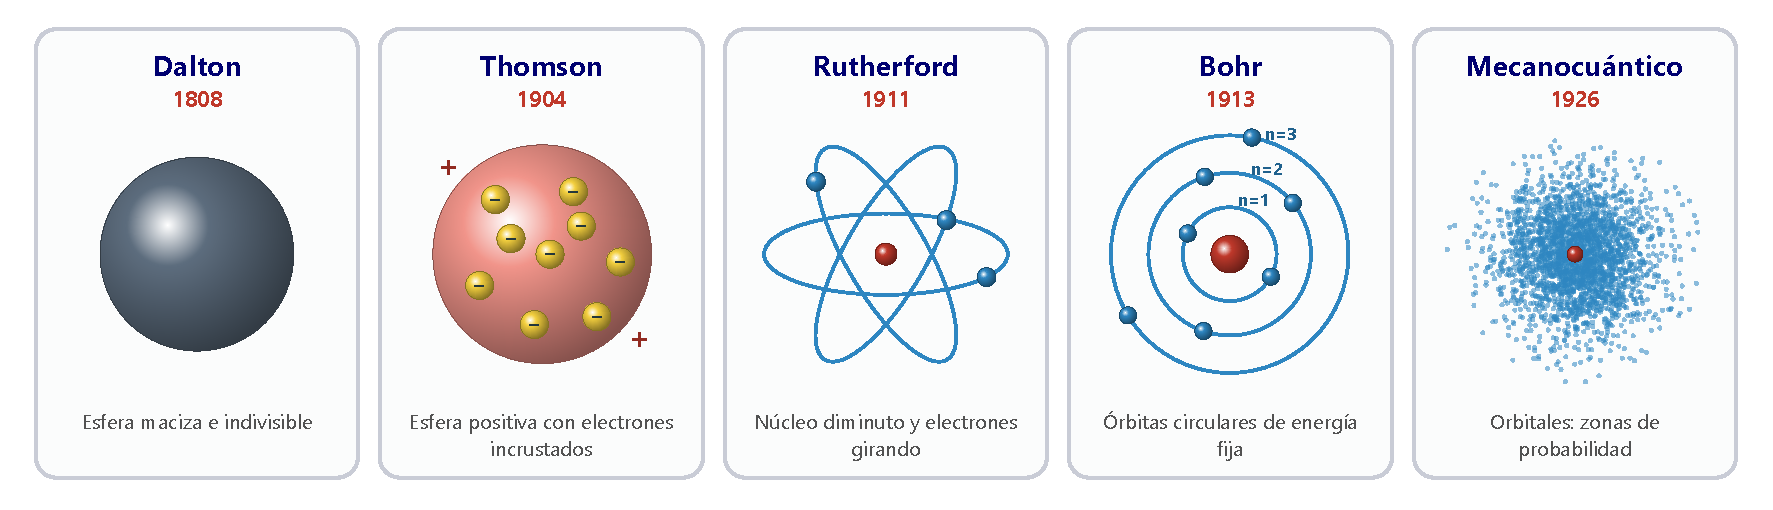
\includegraphics[width=\textwidth]{images/UD3/modelos_atomicos}
    \caption{Evolución de los modelos atómicos.}
    \label{fig:ud3-modelos}
\end{figure}

\subsection{El modelo atómico de Dalton}

Entre 1803 y 1808, \textbf{John Dalton} propuso que los átomos eran \textbf{esferas macizas e indivisibles}, todas iguales
para un mismo elemento y distintas de las de cualquier otro (lo estudiamos en la unidad 1). Este modelo tan sencillo explicaba
las \textbf{leyes ponderales}, pero no contemplaba la existencia de isótopos, predijo mal la fórmula del agua (creyó que era
\ch{HO}) y no podía explicar fenómenos como la electricidad.

\subsection{El descubrimiento del electrón y el modelo de Thomson}

En 1858 se descubrieron los \textbf{rayos catódicos}. Al hacer un vacío casi perfecto en un tubo de vidrio y aplicar una
diferencia de potencial muy alta entre dos electrodos, el \textbf{cátodo} (electrodo negativo) emitía «algo» invisible que
hacía brillar la pared del fondo, recubierta de una sustancia fluorescente. Si se interponía un objeto, su sombra aparecía en la
pantalla: la radiación viajaba en línea recta. En 1897, \textbf{J.\,J. Thomson} estudió a fondo su naturaleza con un tubo como
el de la figura~\ref{fig:ud3-catodicos}.

\begin{figure}[H]
    \centering
    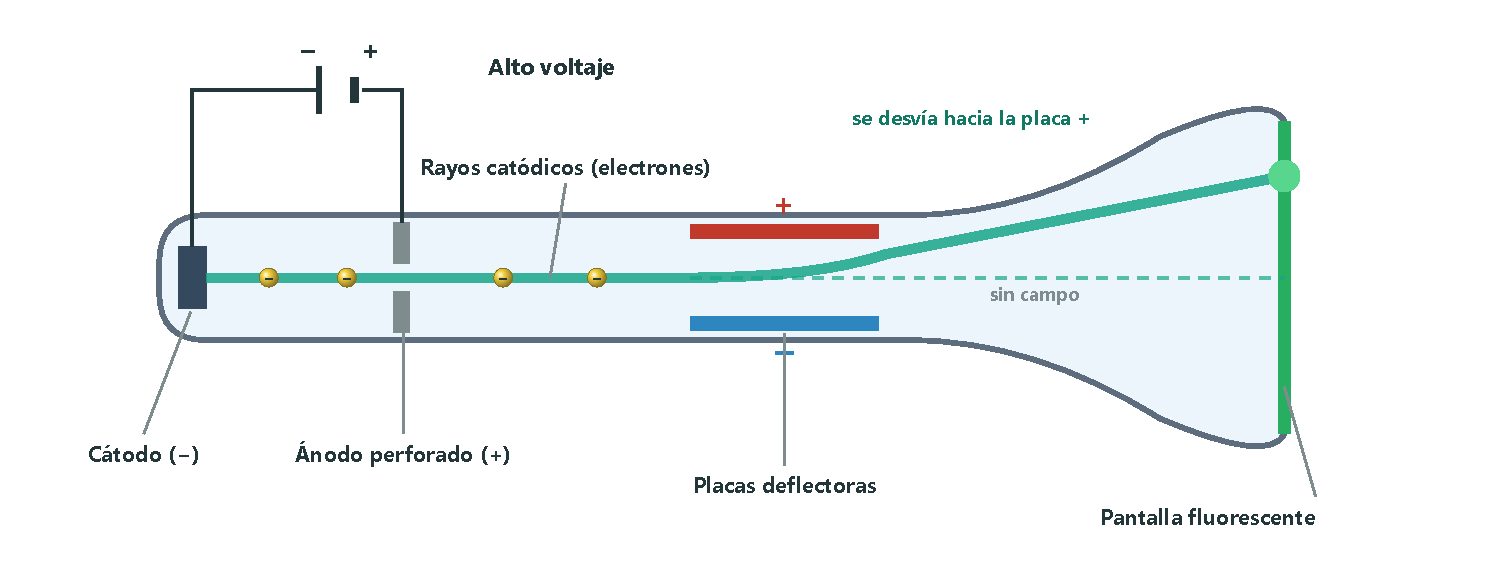
\includegraphics[width=0.85\textwidth]{images/UD3/rayos_catodicos}
    \caption{Tubo de rayos catódicos: las placas cargadas desvían el haz hacia la placa positiva.}
    \label{fig:ud3-catodicos}
\end{figure}

\begin{table}[H]
    \centering
    \caption{Lo que observó Thomson en los rayos catódicos}
    \vspace{-5pt}
    \begin{tabular}{@{}L{7cm}L{7cm}@{}}
        \toprule
        \textbf{Observación} & \textbf{Interpretación} \\
        \midrule
        Hacen girar un pequeño molinillo colocado en su camino & Están formados por \textbf{partículas con masa} \\[3pt]
        Se desvían hacia la placa positiva & Tienen \textbf{carga negativa} \\[3pt]
        Son iguales sea cual sea el metal del cátodo & Son partículas \textbf{fundamentales}, presentes en toda la materia \\[3pt]
        Su relación carga/masa es \(\qty{1.76e11}{\coulomb\per\kilo\gram}\) & Son mucho más \textbf{ligeras} que el átomo más pequeño, el de hidrógeno \\
        \bottomrule
    \end{tabular}
    \label{tab:ud3-thomson}
\end{table}

\begin{definition}[El electrón]
    Thomson concluyó que los rayos catódicos eran partículas con carga negativa, que se llamaron \textbf{electrones}. Su
    existencia demuestra que los átomos \textbf{no son indivisibles}: tienen una estructura interna. Experimentos posteriores
    midieron su carga y su masa:
    \[ q_e = \qty{-1.602e-19}{\coulomb} \qquad\qquad m_e = \qty{9.109e-31}{\kilo\gram} \]
    El electrón no tiene estructura interna: es una \textbf{partícula elemental}.
\end{definition}

En 1909, \textbf{R. Millikan} demostró, con su famoso experimento de la gota de aceite, que cualquier carga eléctrica es un
múltiplo entero de una cantidad mínima, la \textbf{carga elemental}, \(e = \qty{1.602e-19}{\coulomb}\), que es la carga (en
valor absoluto) del electrón.

\paragraph{El modelo de Thomson (1904).} Si los átomos son neutros y contienen electrones, deben tener también carga positiva.
Thomson propuso que el átomo era una \textbf{esfera} con la \textbf{carga positiva repartida uniformemente} en la que estaban
\textbf{incrustados} los electrones, como las pepitas en una sandía. Se le conoce como \emph{modelo del pudin de pasas}. Thomson
recibió el premio Nobel de Física en 1906 por sus investigaciones sobre la conducción de la electricidad en los gases.

\begin{example}
    \textbf{La carga está cuantizada.} En un experimento como el de Millikan se miden las cargas de tres gotas de aceite:
    \(\qty{3.204e-19}{\coulomb}\), \(\qty{4.806e-19}{\coulomb}\) y \(\qty{8.010e-19}{\coulomb}\). ¿Cuántos electrones de exceso
    tiene cada gota?

    \textbf{Solución.} Dividimos cada carga entre la carga elemental:
    \[ \frac{\num{3.204e-19}}{\num{1.602e-19}} = 2; \qquad \frac{\num{4.806e-19}}{\num{1.602e-19}} = 3; \qquad \frac{\num{8.010e-19}}{\num{1.602e-19}} = 5 \]
    Las gotas tienen 2, 3 y 5 electrones de exceso. Nunca se encuentra una carga que no sea un múltiplo entero de \(e\).
\end{example}

\subsection{El modelo atómico de Rutherford}

\paragraph{El experimento de la lámina de oro.} En 1910, \textbf{E. Rutherford} y sus colaboradores \textbf{H. Geiger} y
\textbf{E. Marsden} pusieron a prueba el modelo de Thomson bombardeando una lámina de oro finísima (de una micra de espesor, unas
mil capas de átomos) con \textbf{partículas \(\alpha\)}, de masa \qty{4}{\uma} y carga \(+2e\). Si el modelo de Thomson era
correcto, la masa y la carga estarían repartidas por todo el átomo, como un fluido de muy poca densidad, y las partículas
\(\alpha\), muy rápidas, deberían atravesar la lámina casi sin desviarse. Lo que encontraron fue sorprendente
(figura~\ref{fig:ud3-oro}): casi todas pasaban sin desviarse, pero alrededor de \textbf{una de cada \num{20000} se desviaba más
de \ang{90}}, ¡e incluso alguna rebotaba! Rutherford lo comparó con disparar un proyectil contra una hoja de papel de seda y que
volviera hacia atrás.

\begin{figure}[H]
    \centering
    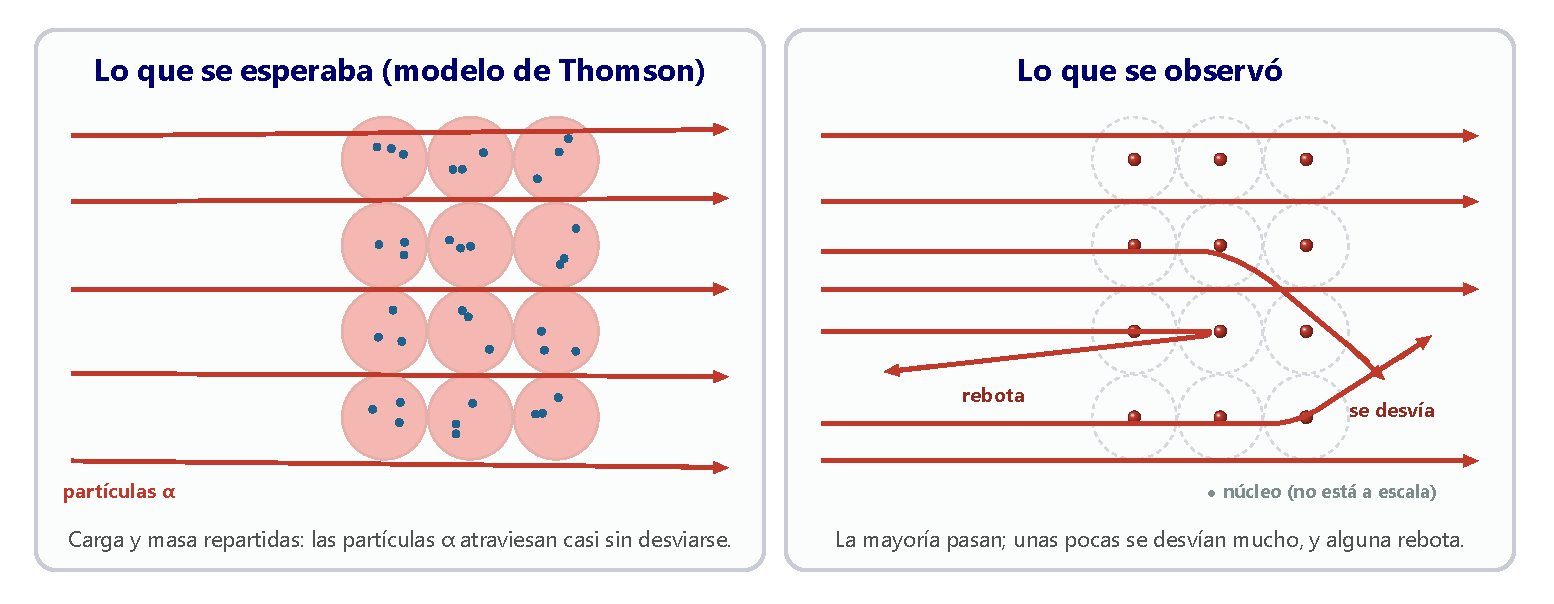
\includegraphics[width=0.9\textwidth]{images/UD3/lamina_oro}
    \caption{Experimento de la lámina de oro: lo que se esperaba y lo que se observó.}
    \label{fig:ud3-oro}
\end{figure}

Rutherford interpretó que en el interior del átomo tenía que haber una zona muy \textbf{densa} y con carga \textbf{positiva},
capaz de repeler y hacer rebotar a las partículas \(\alpha\) que chocaban con ella. Como eso ocurría muy pocas veces, esa zona
debía ser \textbf{pequeñísima} comparada con el átomo.

\begin{definition}[Modelo atómico de Rutherford (1911)]
    \leavevmode % el título de la definición en su propia línea, la lista debajo
    \begin{itemize}
        \item La mayor parte del volumen del átomo está \textbf{vacío}.
        \item En el centro hay un \textbf{núcleo} muy pequeño en el que se concentra casi toda la \textbf{masa} y toda la
        \textbf{carga positiva}.
        \item Los \textbf{electrones} están en la zona exterior, la \textbf{corteza}, \textbf{girando} alrededor del núcleo en
        órbitas circulares, lo que explica que no caigan sobre él a pesar de la atracción eléctrica.
    \end{itemize}
    Por su parecido con el sistema solar se le llama \emph{modelo planetario}.
\end{definition}

\begin{remark}
    \textbf{Un átomo casi vacío.} El radio de un átomo es unas \num{100000} veces mayor que el de su núcleo. Si el núcleo fuera un
    guisante en el centro de un campo de fútbol, los electrones estarían dando vueltas por las gradas.
\end{remark}

\paragraph{El protón.} Ya en 1886 \textbf{E. Goldstein} había detectado rayos con carga positiva en los tubos de descarga, pero
su trabajo tuvo poca repercusión. En 1919, Rutherford obtuvo núcleos de hidrógeno al bombardear nitrógeno con partículas
\(\alpha\), y propuso que el núcleo de hidrógeno, el más pequeño, era una sola partícula con carga positiva, a la que llamó
\textbf{protón}, y que todos los núcleos contenían cierto número de protones:
\(q_p = +e = \qty{1.602e-19}{\coulomb}\) y \(m_p = \qty{1.673e-27}{\kilo\gram}\).

\paragraph{El neutrón.} La masa de los núcleos era mayor que la de sus protones, y además los protones se repelen entre sí. Por
eso Rutherford propuso que en el núcleo había también partículas \textbf{sin carga} y \textbf{con masa}, que lo hicieran estable.
En 1932, \textbf{J. Chadwick} las detectó: era el \textbf{neutrón}, de masa \(m_n = \qty{1.675e-27}{\kilo\gram}\).

\begin{table}[H]
    \centering
    \caption{Partículas subatómicas}
    \vspace{-5pt}
    \begin{tabular}{@{}lccccc@{}}
        \toprule
        \textbf{Partícula} & \textbf{Masa (kg)} & \textbf{Masa (u)} & \textbf{Carga (C)} & \makecell{\textbf{Carga} \\ \textbf{relativa}} & \textbf{Localización} \\
        \midrule
        Electrón, \(e^-\) & \num{9.109e-31} & \num{0.00055} & \num{-1.602e-19} & \(-1\) & Corteza \\[3pt]
        Protón, \(p^+\) & \num{1.673e-27} & \num{1.0073} & \num{+1.602e-19} & \(+1\) & Núcleo \\[3pt]
        Neutrón, \(n\) & \num{1.675e-27} & \num{1.0087} & 0 & 0 & Núcleo \\
        \bottomrule
    \end{tabular}
    \label{tab:ud3-particulas}
\end{table}

\paragraph{Limitaciones del modelo de Rutherford.} El modelo nuclear fue un gran avance (el modelo actual conserva la idea de
núcleo), pero pronto se vieron sus fallos:
\begin{itemize}
    \item Según la física clásica, una carga eléctrica que gira emite radiación y pierde energía. Los electrones irían cayendo en
    espiral hasta chocar con el núcleo: el átomo sería \textbf{inestable}. Sin embargo, la materia es estable.
    \item Los átomos podrían absorber o emitir cualquier cantidad de energía, pero, como veremos, sus espectros son
    \textbf{discontinuos}.
\end{itemize}

\begin{exercise}
    Imagina que lanzas cientos de pelotas de tenis contra una gran cortina y casi todas la atraviesan, pero unas pocas salen
    rebotadas hacia ti. ¿Qué pensarías que hay detrás de la cortina? ¿Qué experimento de la historia de la química se parece a
    esta situación?
    \begin{solu}
        \textcolor{red}{Que detrás hay algunos objetos pequeños y muy duros o pesados} (postes, piedras) y mucho espacio vacío entre
        ellos. Se parece al \textcolor{red}{experimento de la lámina de oro de Rutherford}: las partículas \(\alpha\) que rebotan
        delatan la existencia de un núcleo pequeño, denso y positivo.
    \end{solu}
\end{exercise}

\begin{exercise}
    Imagina que eres uno de los científicos del experimento de la lámina de oro. Al ver los resultados, ¿qué modelo atómico
    propondrías? ¿En qué se diferencia del de Thomson?
    \begin{solu}
        \textcolor{red}{Un modelo con un núcleo central diminuto, positivo y con casi toda la masa, y los electrones fuera, en un
        espacio casi vacío.} En el modelo de Thomson la carga positiva y la masa están repartidas por todo el átomo y los electrones
        están incrustados en ella; en el de Rutherford están separadas en núcleo y corteza.
    \end{solu}
\end{exercise}

\begin{exercise}
    Siempre se habla de Rutherford al mencionar el experimento de la lámina de oro, pero hubo otros científicos que trabajaron con
    él. Investiga quiénes eran y qué otros logros consiguieron, y prepara una infografía.
    \begin{solu}
        \textcolor{red}{Hans Geiger y Ernest Marsden.} \textcolor{blue}{Geiger inventó, con sus alumnos, el contador de radiación
        que lleva su nombre y estudió la relación entre la energía de las partículas \(\alpha\) y la vida media de los núcleos
        radiactivos (ley de Geiger-Nuttall). Marsden, que era todavía estudiante cuando hizo el experimento, se trasladó a Nueva
        Zelanda, donde investigó en física aplicada a la agricultura, y durante la Segunda Guerra Mundial colaboró en el desarrollo
        del radar.}
    \end{solu}
\end{exercise}

\begin{exercise}
    a) Calcula la relación carga/masa del electrón y la del protón. b) ¿Cuántas veces es mayor la masa del protón que la del
    electrón? ¿Por qué decimos que la masa del átomo está en el núcleo?
    \begin{solu}
        a) \(\dfrac{e}{m_e} = \dfrac{\num{1.602e-19}}{\num{9.109e-31}} = \textcolor{red}{\qty{1.76e11}{\coulomb\per\kilo\gram}}\);
        \(\dfrac{e}{m_p} = \dfrac{\num{1.602e-19}}{\num{1.673e-27}} = \textcolor{red}{\qty{9.58e7}{\coulomb\per\kilo\gram}}\).
        b) \(\dfrac{m_p}{m_e} = \textcolor{red}{1837}\). \textcolor{blue}{Protones y neutrones tienen casi 2000 veces más masa que
        los electrones, y están todos en el núcleo.}
    \end{solu}
\end{exercise}

\begin{exercise}
    El radio de un átomo es unas \(10^5\) veces mayor que el de su núcleo. Si hiciéramos una maqueta en la que el núcleo fuera
    una canica de \qty{1}{\cm} de diámetro, ¿qué diámetro tendría el átomo?
    \begin{solu}
        \(\qty{1}{\cm} \cdot 10^5 = \qty{e5}{\cm} = \textcolor{red}{\qty{1}{\km}}\): el átomo sería una esfera de un kilómetro de
        diámetro con una canica en el centro.
    \end{solu}
\end{exercise}

\begin{exercise}
    «Los científicos no dependen de las ideas de un solo hombre, sino de la sabiduría combinada de miles de hombres…», escribió
    Rutherford. ¿Sigue siendo válida esta idea hoy? ¿Por qué es importante colaborar en la investigación científica?
    \begin{solu}
        \textcolor{red}{Respuesta abierta.} \textcolor{blue}{Hoy la ciencia es aún más colaborativa: los grandes avances
        (el bosón de Higgs, las vacunas de ARN, el telescopio James Webb) los firman equipos de cientos o miles de personas de
        muchos países. Cada modelo atómico se apoyó en experimentos y en ideas de otros, como se ve en esta unidad. Hoy diríamos
        «personas», no solo «hombres».}
    \end{solu}
\end{exercise}

\begin{exercise}
    En la historia de los modelos atómicos se mencionan muy pocas mujeres. ¿A qué crees que se debe? Investiga la contribución de
    alguna de ellas, como Harriet Brooks, Marie Curie o Lise Meitner, y escribe un breve informe.
    \begin{solu}
        \textcolor{red}{Respuesta abierta.} \textcolor{blue}{Durante mucho tiempo las mujeres tuvieron muy difícil estudiar en la
        universidad y trabajar en investigación, y su trabajo se atribuía a menudo a sus compañeros. Harriet Brooks, primera mujer
        que trabajó con Rutherford, descubrió el retroceso nuclear y el radón; Marie Curie estudió la radiactividad y descubrió el
        polonio y el radio; Lise Meitner explicó, junto con Otto Frisch, la fisión nuclear.}
    \end{solu}
\end{exercise}

%========================================================================================
\section{La masa de los átomos}\label{sec:ud3-masa}
%========================================================================================

\subsection{Número atómico y número másico}

\begin{definition}[Número atómico y número másico]
    \leavevmode % el título de la definición en su propia línea, la lista debajo
    \begin{itemize}
        \item El \textbf{número atómico}, \(Z\), es el número de \textbf{protones} del núcleo. Todos los átomos con el mismo
        número atómico tienen las mismas propiedades químicas: un \textbf{elemento químico} es una sustancia formada por átomos con
        el mismo \(Z\).
        \item El \textbf{número másico}, \(A\), es el número de \textbf{nucleones} (protones más neutrones) del núcleo:
        \[ A = Z + N \qquad (N = \text{número de neutrones}) \]
    \end{itemize}
    Un átomo se representa \(^{A}_{Z}\mathrm{X}\), donde X es el símbolo del elemento; si es un ion, su carga neta se escribe
    arriba a la derecha.
\end{definition}

\begin{example}
    \textbf{Partículas de un átomo.} Indica el número másico, el número atómico y el número de protones, neutrones y electrones
    del isótopo \ch{^{238}_{92}U}.

    \textbf{Solución.} De la notación leemos directamente \(Z = 92\) y \(A = 238\). El número de protones es el número atómico:
    \(p = 92\). Los neutrones: \(N = A - Z = 238 - 92 = 146\). Como el átomo es neutro, tiene tantos electrones como protones:
    92 electrones.
\end{example}

\subsection{Isótopos}

\begin{definition}[Isótopos]
    Son átomos de un mismo elemento (igual número de \textbf{protones}) con distinto número de \textbf{neutrones}, es decir,
    con el mismo \(Z\) y distinto \(A\). La palabra viene del griego \emph{isos}, «igual», y \emph{topos}, «lugar»: ocupan el
    mismo lugar en la tabla periódica.
\end{definition}

La mayoría de los elementos naturales son mezclas de varios isótopos. Como tienen los mismos electrones, su comportamiento
químico es el mismo, aunque algunas propiedades físicas (la masa, la densidad, la estabilidad del núcleo) son distintas. El
oxígeno, por ejemplo, tiene tres isótopos estables: \ch{^{16}_{8}O}, \ch{^{17}_{8}O} y \ch{^{18}_{8}O}; el hidrógeno tiene los
tres de la figura~\ref{fig:ud3-isotopos}. La \textbf{abundancia isotópica} es el porcentaje de átomos de un isótopo que hay en
una muestra natural del elemento.

\begin{figure}[H]
    \centering
    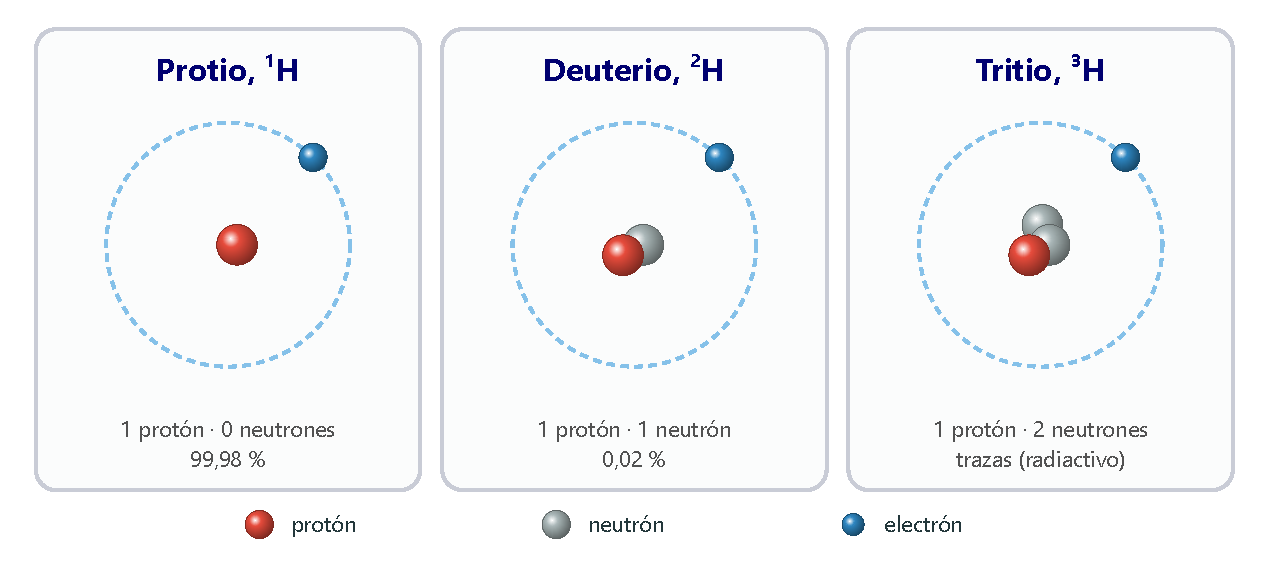
\includegraphics[width=0.72\textwidth]{images/UD3/isotopos}
    \caption{Los tres isótopos del hidrógeno (el núcleo no está a escala).}
    \label{fig:ud3-isotopos}
\end{figure}

\begin{exercise}
    Indica el número de protones, neutrones y electrones de: \ch{^{119}_{50}Sn^4+}, \ch{^{37}_{17}Cl^-}, \ch{^{107}_{47}Ag^+},
    \ch{^{59}_{27}Co^2+} y \ch{^{238}_{92}U}.
    \begin{solu}
        \begin{tabular}{@{}lccccc@{}}
            \toprule
            & \ch{^{119}_{50}Sn^4+} & \ch{^{37}_{17}Cl^-} & \ch{^{107}_{47}Ag^+} & \ch{^{59}_{27}Co^2+} & \ch{^{238}_{92}U} \\
            \midrule
            Protones & 50 & 17 & 47 & 27 & 92 \\[3pt]
            Neutrones & 69 & 20 & 60 & 32 & 146 \\[3pt]
            Electrones & \textcolor{red}{46} & \textcolor{red}{18} & \textcolor{red}{46} & \textcolor{red}{25} & \textcolor{red}{92} \\
            \bottomrule
        \end{tabular}
    \end{solu}
\end{exercise}

\begin{exercise}
    De los átomos \ch{^{12}_{6}C}, \ch{^{14}_{6}C}, \ch{^{14}_{7}N}, \ch{^{40}_{18}Ar} y \ch{^{40}_{20}Ca}, ¿cuáles son isótopos
    entre sí? ¿Cuáles tienen el mismo número másico? ¿Cuáles tienen el mismo número de neutrones?
    \begin{solu}
        \textcolor{red}{Isótopos: \ch{^{12}C} y \ch{^{14}C}} (mismo \(Z\)). \textcolor{red}{Mismo \(A\): \ch{^{14}C} y \ch{^{14}N};
        \ch{^{40}Ar} y \ch{^{40}Ca}.} Neutrones: 6, 8, 7, 22 y 20: \textcolor{red}{ninguno coincide}.
    \end{solu}
\end{exercise}

\subsection{La masa atómica}

La masa atómica de un elemento se calcula con mucha precisión a partir de su \textbf{espectro de masas}.

\paragraph{Espectrometría de masas.} Es una técnica de análisis que permite \textbf{separar las partículas} de una muestra
(átomos, moléculas o fragmentos de moléculas) \textbf{según su masa}. Un \textbf{espectrómetro de masas}
(figura~\ref{fig:ud3-espectrometro}) tiene tres partes:
\begin{itemize}
    \item \textbf{Fuente de iones}: la muestra, en estado gaseoso, se \textbf{ioniza}; normalmente todos los iones adquieren la
    misma carga. Después, unas placas cargadas los aceleran.
    \item \textbf{Analizador}: los iones atraviesan un \textbf{campo magnético} que curva su trayectoria. El radio de la curva
    depende de la masa de cada ion: los más ligeros se desvían más. Así, el haz inicial se \textbf{separa} en tantos haces como
    masas distintas había en la muestra.
    \item \textbf{Detector}: recoge cada haz por separado y mide el \textbf{número de iones} que llegan.
\end{itemize}

\begin{figure}[H]
    \centering
    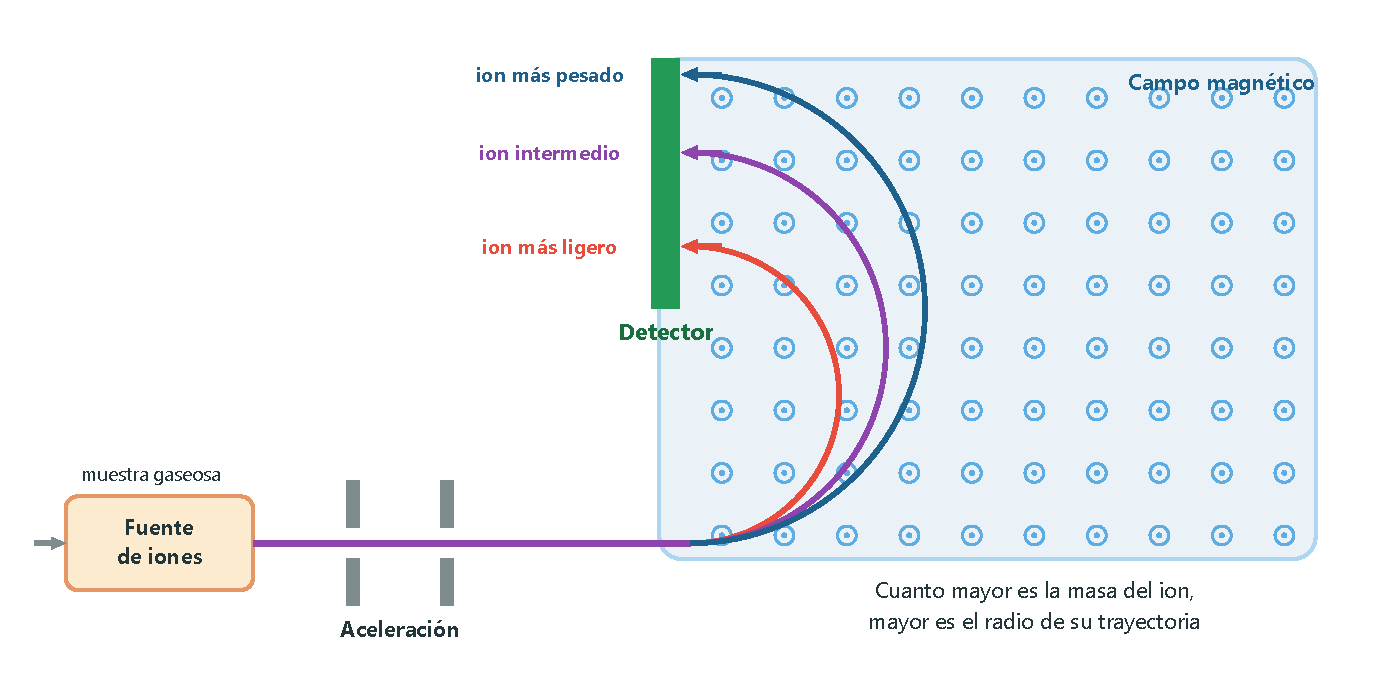
\includegraphics[width=0.7\textwidth]{images/UD3/espectrometro}
    \caption{Esquema de un espectrómetro de masas.}
    \label{fig:ud3-espectrometro}
\end{figure}

El resultado es el \textbf{espectro de masas} (figura~\ref{fig:ud3-espectro-cl}): cada pico indica la \textbf{masa} de un tipo
de partícula y su altura, la \textbf{abundancia relativa} (el porcentaje de cada partícula en la muestra).

\begin{figure}[H]
    \centering
    \begin{tikzpicture}
        \begin{axis}[grafica, width=0.55\linewidth, height=5cm, ybar, bar width=5pt, xmin=33.5, xmax=38.5, ymin=0, ymax=90,
            xtick={34,35,36,37,38}, xlabel={Masa isotópica (u)}, ylabel={Abundancia (\%)}, grid=none,
            nodes near coords, nodes near coords style={font=\scriptsize, /pgf/number format/use comma}]
            \addplot[fill=ocre!70, draw=ocre] coordinates {(34.969,75.78) (36.966,24.22)};
        \end{axis}
    \end{tikzpicture}
    \caption{Espectro de masas del cloro: dos isótopos, \ch{^{35}Cl} y \ch{^{37}Cl}.}
    \label{fig:ud3-espectro-cl}
\end{figure}

\begin{definition}[Masa atómica de un elemento]
    Es la \textbf{media ponderada} de las masas de sus isótopos, según su abundancia:
    \[ \bar{A} = \frac{\sum A_i \cdot \%_i}{100} = \frac{A_1 \cdot \%_1 + A_2 \cdot \%_2 + \dots}{100} \]
    donde \(A_i\) es la masa del isótopo \(i\) (en u) y \(\%_i\), su abundancia relativa. Por eso las masas atómicas de la tabla
    periódica no son números enteros.
\end{definition}

\begin{example}
    \textbf{Masa atómica del silicio.} El silicio natural está formado por \ch{^{28}Si} (\qty{27.977}{\uma}; 92,2\,\%),
    \ch{^{29}Si} (\qty{28.976}{\uma}; 4,7\,\%) y \ch{^{30}Si} (\qty{29.974}{\uma}). Calcula su masa atómica.

    \textbf{Solución.} Primero, la abundancia que falta: \(100 - (\num{92.2} + \num{4.7}) = \qty{3.1}{\percent}\) de \ch{^{30}Si}.
    \[ \bar{A} = \frac{\num{27.977} \cdot \num{92.2} + \num{28.976} \cdot \num{4.7} + \num{29.974} \cdot \num{3.1}}{100} = \qty{28.09}{\uma} \]
    El resultado está muy cerca de 28, porque casi todo el silicio es \ch{^{28}Si}.
\end{example}

\begin{example}
    \textbf{Abundancias a partir de la masa atómica.} El boro tiene dos isótopos, \ch{^{10}B} (\qty{10.013}{\uma}) y \ch{^{11}B}
    (\qty{11.009}{\uma}), y su masa atómica es \qty{10.81}{\uma}. Calcula la abundancia de cada uno.

    \textbf{Solución.} Si \(x\) es el porcentaje de \ch{^{10}B}, el de \ch{^{11}B} es \(100 - x\):
    \[ \num{10.81} = \frac{\num{10.013}\,x + \num{11.009}\,(100 - x)}{100} \;\Rightarrow\; 1081 = 1100{,}9 - \num{0.996}\,x
    \;\Rightarrow\; x = \num{19.98} \]
    Hay un 20,0\,\% de \ch{^{10}B} y un 80,0\,\% de \ch{^{11}B}.
\end{example}

\begin{exercise}
    El galio tiene dos isótopos: \ch{^{69}Ga}, de \qty{68.926}{\uma} y 60,11\,\% de abundancia, y \ch{^{71}Ga}, de
    \qty{70.925}{\uma} y 39,89\,\%. Calcula la masa atómica del galio y dibuja su espectro de masas.
    \begin{solu}
        \(\bar{A} = \dfrac{\num{68.926} \cdot \num{60.11} + \num{70.925} \cdot \num{39.89}}{100} = \textcolor{red}{\qty{69.72}{\uma}}\).
        \textcolor{blue}{El espectro tiene dos picos, en 68,9 y en 70,9, de alturas 60,11 y 39,89.}
    \end{solu}
\end{exercise}

\begin{exercise}
    Calcula la masa atómica de: a) el cobre: \ch{^{63}Cu}, \qty{62.93}{\uma}, 69,17\,\%; \ch{^{65}Cu}, \qty{64.93}{\uma},
    30,83\,\%; b) el cloro, con los datos de la figura~\ref{fig:ud3-espectro-cl}.
    \begin{solu}
        a) \(\dfrac{\num{62.93} \cdot \num{69.17} + \num{64.93} \cdot \num{30.83}}{100} = \textcolor{red}{\qty{63.55}{\uma}}\).
        b) \(\dfrac{\num{34.969} \cdot \num{75.78} + \num{36.966} \cdot \num{24.22}}{100} = \textcolor{red}{\qty{35.45}{\uma}}\).
    \end{solu}
\end{exercise}

\begin{exercise}
    El argón tiene tres isótopos estables: \ch{^{36}Ar} (\qty{35.968}{\uma}; 0,337\,\%), \ch{^{38}Ar} (\qty{37.963}{\uma};
    0,063\,\%) y \ch{^{40}Ar} (\qty{39.962}{\uma}; 99,600\,\%). Calcula su masa atómica. ¿Por qué el argón (\(Z = 18\)) tiene
    mayor masa atómica que el potasio (\(Z = 19\), \qty{39.10}{\uma})?
    \begin{solu}
        \(\bar{A} = \dfrac{\num{35.968} \cdot \num{0.337} + \num{37.963} \cdot \num{0.063} + \num{39.962} \cdot \num{99.600}}{100} =
        \textcolor{red}{\qty{39.95}{\uma}}\). \textcolor{red}{Porque el isótopo más abundante del argón tiene 22 neutrones}, y el
        del potasio (\ch{^{39}K}), solo 20. La masa no depende solo de \(Z\): por eso la tabla se ordena por número atómico y no por
        masa.
    \end{solu}
\end{exercise}

%========================================================================================
\section{Interacción de la radiación electromagnética con la materia}\label{sec:ud3-radiacion}
%========================================================================================

La forma en que la luz y las demás ondas electromagnéticas interaccionan con la materia nos da mucha información sobre la
estructura interna de los átomos. Veamos primero qué son estas ondas.

\subsection{Ondas electromagnéticas}

En el siglo XIX hubo una larga discusión sobre si la luz era un haz de partículas o una onda, que pareció zanjarse a favor de la
teoría ondulatoria. En 1865, \textbf{J.\,C. Maxwell} demostró teóricamente que un campo eléctrico y uno magnético acoplados se
propagan en forma de \textbf{onda}, incluso en el \textbf{vacío}, a unos \qty{300000}{\km\per\s}: la velocidad de la luz. Las
\textbf{ondas electromagnéticas} transportan energía mediante la variación sinusoidal de un campo eléctrico y otro magnético
perpendiculares. En 1887, \textbf{H. Hertz} las generó y las detectó en el laboratorio, confirmando las predicciones de Maxwell.

\begin{figure}[H]
    \centering
    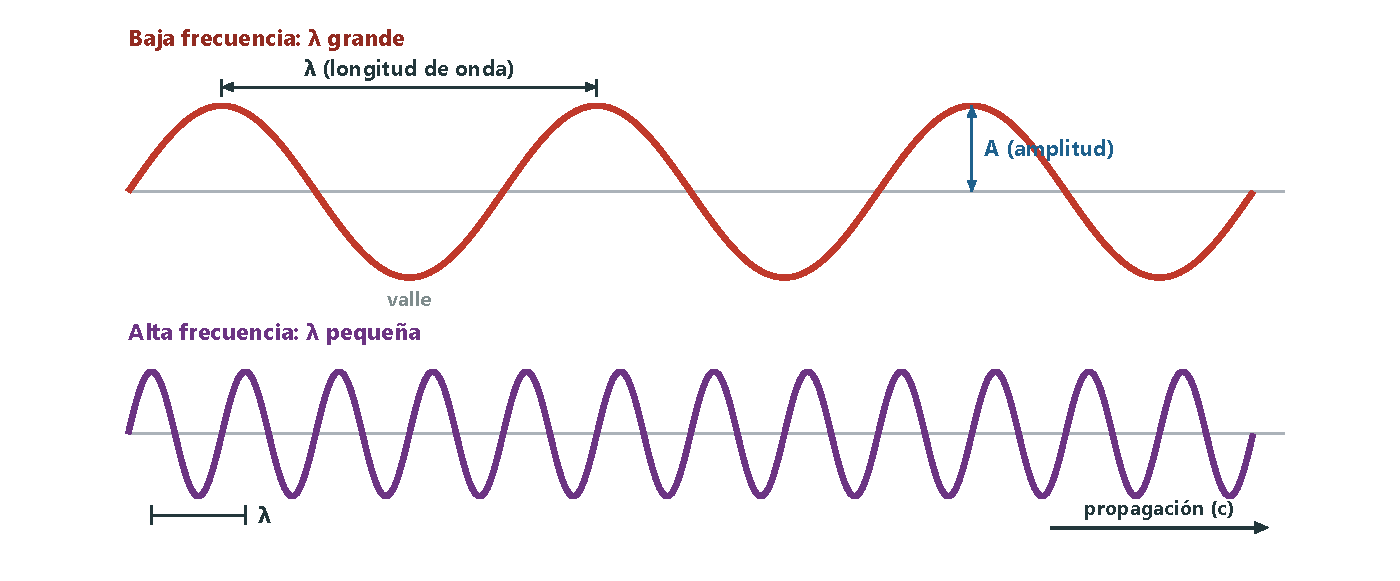
\includegraphics[width=0.7\textwidth]{images/UD3/onda}
    \caption{Longitud de onda y amplitud de una onda. Cuanto mayor es la frecuencia, menor es la longitud de onda.}
    \label{fig:ud3-onda}
\end{figure}

\begin{table}[H]
    \centering
    \caption{Magnitudes de una onda}
    \vspace{-5pt}
    \begin{tabular}{@{}lcL{8.2cm}@{}}
        \toprule
        \textbf{Magnitud} & \makecell{\textbf{Símbolo} \\ \textbf{(unidad SI)}} & \textbf{Significado} \\
        \midrule
        Longitud de onda & \(\lambda\) (\unit{\m}) & Distancia entre dos crestas consecutivas \\[3pt]
        Periodo & \(T\) (\unit{\s}) & Tiempo que tarda la onda en avanzar una longitud de onda \\[3pt]
        Frecuencia & \(\nu\) (\unit{\hertz} = \unit{\per\s}) & Número de ondas que pasan por un punto en cada segundo (hercio, en honor a Hertz) \\[3pt]
        Número de onda & \(\tilde{\nu}\) (\unit{\per\m}) & Número de longitudes de onda que caben en una unidad de longitud \\[3pt]
        Velocidad de propagación & \(c\) (\unit{\m\per\s}) & Distancia que avanza la onda en cada segundo; en el vacío, \(c = \qty{3.00e8}{\m\per\s}\) \\
        \bottomrule
    \end{tabular}
    \label{tab:ud3-magnitudes}
\end{table}

Estas magnitudes están relacionadas:
\[ \nu = \frac{1}{T} \qquad\qquad \tilde{\nu} = \frac{1}{\lambda} \qquad\qquad c = \frac{\lambda}{T} = \lambda \cdot \nu \]

\begin{example}
    \textbf{Televisión UHF.} Las antiguas televisiones sintonizaban la banda UHF, que ocupa frecuencias entre 300 MHz y 3 GHz.
    ¿Qué longitud de onda tiene una emisión de \qty{600}{\mega\hertz}?

    \textbf{Solución.} \(\lambda = \dfrac{c}{\nu} = \dfrac{\qty{3.00e8}{\m\per\s}}{\qty{600e6}{\hertz}} = \qty{0.500}{\m} = \qty{50.0}{\cm}\).
\end{example}

\subsection{El espectro electromagnético}

\begin{definition}[Espectro electromagnético]
    Es el conjunto de todas las ondas electromagnéticas, ordenadas según su frecuencia o su longitud de onda. La
    \textbf{energía} que transporta una onda es tanto mayor cuanto mayor es su \textbf{frecuencia} (y menor su longitud de onda).
\end{definition}

La \textbf{luz visible} es solo una pequeña parte del espectro, con longitudes de onda entre unos \qty{380}{\nm} (violeta) y
\qty{750}{\nm} (rojo) (figura~\ref{fig:ud3-espectro-em}). Las radiaciones más energéticas que el visible (ultravioleta, rayos X
y gamma) pueden arrancar electrones a los átomos: son \textbf{ionizantes}, y por eso peligrosas para los seres vivos.

\begin{figure}[H]
    \centering
    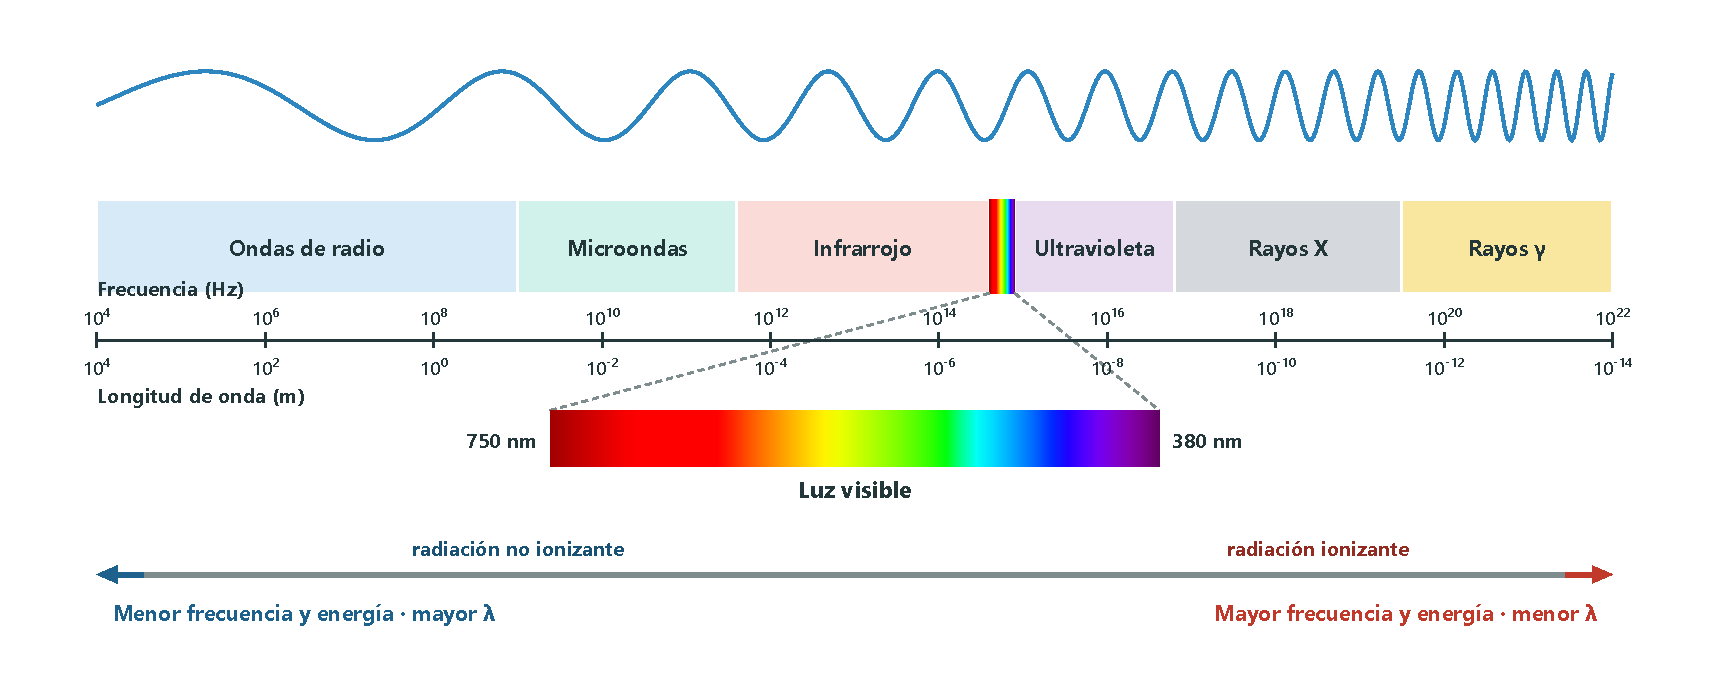
\includegraphics[width=\textwidth]{images/UD3/espectro_em}
    \caption{El espectro electromagnético.}
    \label{fig:ud3-espectro-em}
\end{figure}

\begin{exercise}
    Un teléfono móvil emite y recibe una señal de \qty{900}{\mega\hertz}. ¿Cuál es su longitud de onda?
    \begin{solu}
        \(\lambda = \dfrac{\num{3.00e8}}{\num{9.00e8}} = \textcolor{red}{\qty{0.333}{\m} = \qty{33.3}{\cm}}\).
    \end{solu}
\end{exercise}

\begin{exercise}
    Al pasar un haz de luz blanca por un prisma se descompone en los colores del arcoíris. ¿Por qué se llama a esa zona
    \emph{espectro visible}? Calcula su intervalo de frecuencias.
    \begin{solu}
        \textcolor{red}{Porque es la única parte del espectro que detecta el ojo humano.} \(\nu = c/\lambda\):
        \(\dfrac{\num{3.00e8}}{\num{750e-9}} = \qty{4.0e14}{\hertz}\) (rojo) y \(\dfrac{\num{3.00e8}}{\num{380e-9}} = \qty{7.9e14}{\hertz}\)
        (violeta): \textcolor{red}{entre \num{4.0e14} y \qty{7.9e14}{\hertz}}.
    \end{solu}
\end{exercise}

\begin{exercise}
    ¿Es correcto decir que la luz infrarroja es visible? ¿Cómo es posible entonces que las cámaras térmicas «vean» a las personas
    en la oscuridad?
    \begin{solu}
        \textcolor{red}{No: su longitud de onda es mayor que la del rojo y nuestro ojo no la detecta.} Todos los cuerpos emiten
        radiación infrarroja según su temperatura; \textcolor{red}{las cámaras térmicas tienen sensores sensibles al infrarrojo} y
        la convierten en una imagen visible.
    \end{solu}
\end{exercise}

\subsection{Espectros atómicos}

La materia \textbf{absorbe} radiación, y el efecto que produce depende de la frecuencia y del tipo de materia: las moléculas de
agua de los alimentos absorben microondas y se agitan, y el rozamiento con las moléculas cercanas calienta la comida. La materia
también \textbf{emite} radiación, con una frecuencia que depende de la temperatura: el filamento de las antiguas bombillas,
muy caliente, emitía luz visible.

En 1859, \textbf{R. Bunsen} y \textbf{G. Kirchhoff} idearon el \textbf{espectroscopio}, un aparato que separa, con un prisma o
una red de difracción, las radiaciones de distinta frecuencia que forman un haz.
\begin{itemize}
    \item En la \textbf{espectroscopía de absorción} se hace pasar luz blanca a través de una muestra gaseosa y se analiza la luz
    que sale: se obtiene el \textbf{espectro de absorción}.
    \item En la \textbf{espectroscopía de emisión} se analiza la radiación que emite una sustancia excitada (calentada o sometida a
    una descarga eléctrica): es su \textbf{espectro de emisión}.
\end{itemize}

Con el modelo de Rutherford no había ninguna limitación para la energía del electrón, así que se esperaba que los espectros
fueran \textbf{continuos}: que los átomos absorbieran o emitieran radiación de todas las frecuencias. No es así: los espectros
atómicos son \textbf{discontinuos}. Los átomos solo absorben unas frecuencias determinadas, que aparecen como rayas negras en el
espectro de absorción, y al excitarlos emiten justamente esas mismas frecuencias, que aparecen como rayas de colores en el de
emisión (figura~\ref{fig:ud3-espectros}).

\begin{figure}[H]
    \centering
    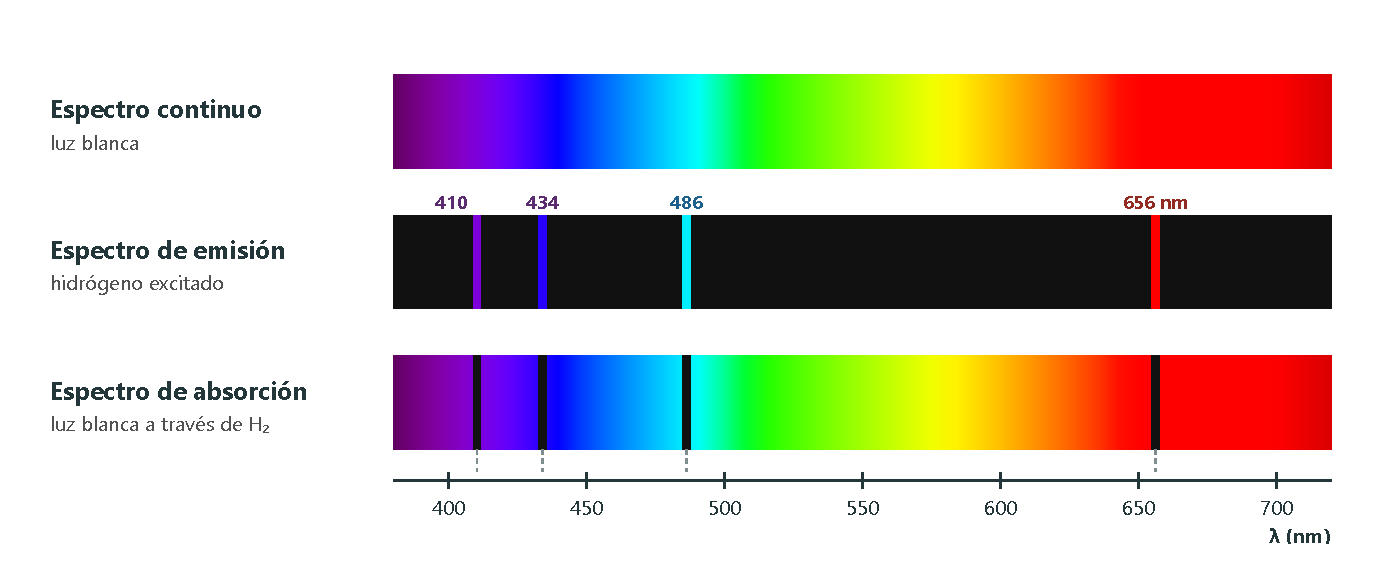
\includegraphics[width=0.8\textwidth]{images/UD3/espectros_atomicos}
    \caption{Espectro continuo y espectros de emisión y de absorción del hidrógeno en la zona visible.}
    \label{fig:ud3-espectros}
\end{figure}

\begin{remark}
    Las frecuencias que absorbe o emite un átomo son \textbf{características} de cada elemento: su espectro es como su
    \textbf{huella dactilar}. Gracias a ello se descubrieron elementos nuevos (el cesio, el rubidio o el helio, que se encontró
    en el espectro del Sol antes que en la Tierra) y hoy se analiza la composición de las estrellas o de una muestra de suelo.
\end{remark}

\paragraph{Series espectrales del hidrógeno.} En 1885, \textbf{J.\,J. Balmer} encontró una fórmula matemática para las rayas
visibles del espectro del hidrógeno, y en 1890 \textbf{J. Rydberg} la generalizó para todas las series que se fueron
descubriendo después:
\[ \frac{1}{\lambda} = R \left( \frac{1}{n_1^2} - \frac{1}{n_2^2} \right) \qquad (n_2 > n_1) \]
donde \(R = \qty{1.097e7}{\per\m}\) es la \textbf{constante de Rydberg}, y \(n_1\) y \(n_2\) son números enteros. Cada valor de
\(n_1\) da una serie de rayas:

\begin{table}[H]
    \centering
    \caption{Series espectrales del hidrógeno}
    \vspace{-5pt}
    \begin{tabular}{@{}lccc@{}}
        \toprule
        \textbf{Serie} & \textbf{Año} & \(\boldsymbol{n_1}\) & \textbf{Zona del espectro} \\
        \midrule
        Lyman & 1906 & 1 & Ultravioleta \\[3pt]
        Balmer & 1885 & 2 & Visible \\[3pt]
        Paschen & 1908 & 3 & Infrarrojo \\[3pt]
        Brackett & 1922 & 4 & Infrarrojo \\[3pt]
        Pfund & 1924 & 5 & Infrarrojo \\
        \bottomrule
    \end{tabular}
    \label{tab:ud3-series}
\end{table}

\begin{example}
    \textbf{Primera raya de la serie de Lyman.} Calcula la longitud de onda de la raya de la serie de Lyman con \(n_2 = 2\). ¿En
    qué zona del espectro está?

    \textbf{Solución.} \(\dfrac{1}{\lambda} = \num{1.097e7} \left( \dfrac{1}{1^2} - \dfrac{1}{2^2} \right) = \num{1.097e7} \cdot
    \num{0.75} = \qty{8.23e6}{\per\m}\), así que \(\lambda = \qty{1.215e-7}{\m} = \qty{121.5}{\nm}\): está en el
    \textbf{ultravioleta}, fuera del visible.
\end{example}

\begin{exercise}
    Calcula la longitud de onda de la raya de la serie de Paschen que corresponde a \(n_2 = 5\).
    \begin{solu}
        \(\dfrac{1}{\lambda} = \num{1.097e7} \left( \dfrac{1}{9} - \dfrac{1}{25} \right) = \qty{7.80e5}{\per\m}\):
        \(\lambda = \textcolor{red}{\qty{1.28e-6}{\m} = \qty{1282}{\nm}}\) (infrarrojo).
    \end{solu}
\end{exercise}

\begin{exercise}
    Una de las rayas de la serie de Balmer tiene una longitud de onda de \qty{486}{\nm}. ¿Cuál es el valor de \(n_2\)?
    \begin{solu}
        \(\dfrac{1}{n_2^2} = \dfrac{1}{4} - \dfrac{1}{R \lambda} = \num{0.25} - \dfrac{1}{\num{1.097e7} \cdot \num{486e-9}} = \num{0.0624}\):
        \(n_2^2 = 16\), \(\textcolor{red}{n_2 = 4}\).
    \end{solu}
\end{exercise}

\subsection{La hipótesis de Planck}

La física clásica, según la cual una radiación de cualquier frecuencia podía intercambiar cualquier cantidad de energía con la
materia, no conseguía explicar los espectros atómicos ni la radiación que emiten los cuerpos calientes.

\begin{definition}[Hipótesis de Planck (1900)]
    \textbf{Max Planck} propuso que los átomos no absorben ni emiten energía de forma continua, sino en \textbf{paquetes}
    indivisibles a los que llamó \textbf{cuantos}. La energía de un cuanto de radiación, o \textbf{fotón}, es:
    \[ E = h \cdot \nu = \frac{h \cdot c}{\lambda} \]
    donde \(\nu\) es la frecuencia de la radiación y \(h = \qty{6.626e-34}{\joule\s}\) es la \textbf{constante de Planck}.
\end{definition}

Planck, que recibió el premio Nobel en 1918, propuso su hipótesis casi como un «truco» matemático para explicar la radiación
de un cuerpo caliente. Pero en 1905 \textbf{A. Einstein} la usó para explicar el \textbf{efecto fotoeléctrico} (la emisión de
electrones de un metal iluminado con luz de frecuencia suficiente), y se vio que era el comienzo de una física nueva: la
\textbf{física cuántica}.

\begin{example}
    \textbf{Energía de un fotón.} El espectro de emisión del helio tiene una raya verde de \qty{501.6}{\nm}. a) ¿Cuál es la energía
    de uno de sus fotones? b) ¿Y la de un mol de fotones?

    \textbf{Solución.} a) Pasamos la longitud de onda a metros y aplicamos la ecuación de Planck:
    \[ E = \frac{h c}{\lambda} = \frac{\qty{6.626e-34}{\joule\s} \cdot \qty{3.00e8}{\m\per\s}}{\qty{501.6e-9}{\m}} = \qty{3.96e-19}{\joule} \]
    b) \(E = \qty{3.96e-19}{\joule}/\text{fotón} \cdot \num{6.022e23}\ \text{fotones}/\unit{\mol} = \qty{2.39e5}{\joule\per\mol} =
    \qty{239}{\kilo\joule\per\mol}\).
\end{example}

\paragraph{La doble naturaleza de la radiación.} Hoy admitimos que la radiación electromagnética, incluida la luz, tiene una
naturaleza \textbf{dual}: se \textbf{propaga} como una \textbf{onda} (por eso se refleja, se refracta o se difracta) e
\textbf{interacciona} con la materia como un conjunto de partículas, los \textbf{fotones}. Los dos aspectos son
complementarios, pero nunca se manifiestan a la vez.

\begin{exercise}
    Calcula la energía de un fotón de las microondas de un horno (\qty{2.45}{\giga\hertz}) y la de un fotón de radiación
    ultravioleta de \qty{250}{\nm}. ¿Por qué la radiación ultravioleta puede dañar el ADN de las células y las microondas no?
    \begin{solu}
        Microondas: \(E = h \nu = \num{6.626e-34} \cdot \num{2.45e9} = \textcolor{red}{\qty{1.62e-24}{\joule}}\). Ultravioleta:
        \(E = \dfrac{h c}{\lambda} = \textcolor{red}{\qty{7.95e-19}{\joule}}\), unas \num{500000} veces más.
        \textcolor{blue}{Un fotón ultravioleta tiene energía suficiente para romper enlaces químicos; los de microondas solo hacen
        vibrar o girar las moléculas (calientan), aunque haya muchísimos.}
    \end{solu}
\end{exercise}

\begin{exercise}
    Explica a un compañero que ha faltado a clase la diferencia entre un espectro continuo, uno de emisión y uno de absorción.
    \begin{solu}
        \textcolor{red}{El continuo contiene todas las frecuencias} (la luz blanca del Sol o de un filamento muy caliente).
        \textcolor{red}{El de emisión son rayas de colores sobre fondo negro}: las frecuencias que emite un elemento excitado.
        \textcolor{red}{El de absorción es un espectro continuo con rayas negras}: las frecuencias que absorbe el elemento al pasar
        la luz a través de él. Las rayas de ambos están en las mismas posiciones.
    \end{solu}
\end{exercise}

%========================================================================================
\section{Hacia el modelo actual del átomo}\label{sec:ud3-actual}
%========================================================================================

A medida que la física cuántica avanzaba y mejoraban los instrumentos de laboratorio, se fue conociendo mejor la estructura del
átomo.

\subsection{El modelo atómico de Bohr}

En 1913, \textbf{Niels Bohr} mejoró el modelo de Rutherford incorporándole la teoría cuántica de Planck.

\begin{definition}[Postulados de Bohr]
    \leavevmode % el título de la definición en su propia línea, la lista debajo
    \begin{enumerate}
        \item Los electrones giran alrededor del núcleo en ciertas \textbf{órbitas circulares estacionarias}, en las que
        \textbf{no emiten energía}, aunque sean cargas aceleradas.
        \item La energía del electrón está \textbf{cuantizada}: solo puede tomar ciertos valores, que dependen del
        \textbf{número cuántico principal}, \(n = 1, 2, 3\dots\) La órbita de menor energía, la más cercana al núcleo, es la del
        \textbf{nivel} \(n = 1\).
        \item El electrón puede \textbf{cambiar de órbita} absorbiendo o emitiendo un \textbf{fotón} cuya energía es igual a la
        diferencia de energía entre los dos niveles (figura~\ref{fig:ud3-foton}):
        \[ |\Delta E| = E_{\text{fotón}} = |E_{\text{final}} - E_{\text{inicial}}| = h \cdot \nu = \frac{h c}{\lambda} \]
    \end{enumerate}
\end{definition}

\begin{figure}[H]
    \centering
    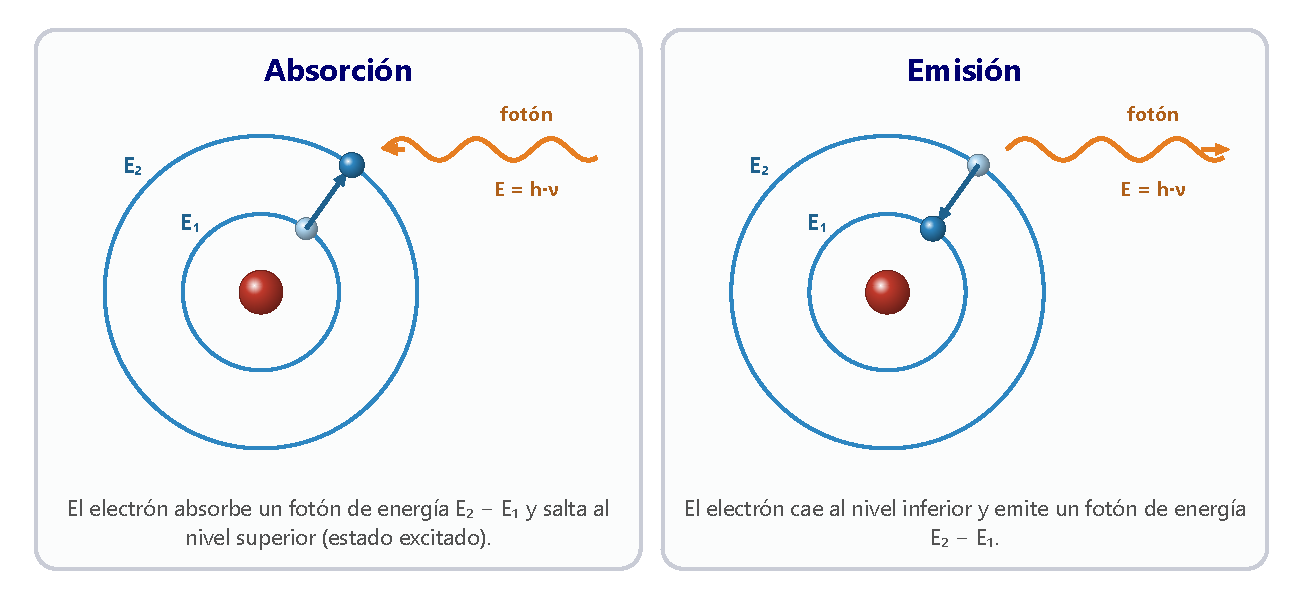
\includegraphics[width=0.72\textwidth]{images/UD3/bohr_foton}
    \caption{Explicación de Bohr para la absorción y la emisión de energía.}
    \label{fig:ud3-foton}
\end{figure}

Para el átomo de hidrógeno, Bohr calculó la energía de cada nivel:
\[ E_n = -\frac{\qty{2.18e-18}{\joule}}{n^2} = -\frac{\qty{13.6}{\electronvolt}}{n^2} \]
La energía es negativa porque se toma como cero la del electrón libre, fuera del átomo (\(n = \infty\)): para separar el
electrón del núcleo hay que darle energía. Con esta expresión se deduce la fórmula de Rydberg, lo que supuso un gran éxito del
modelo.

\paragraph{Interpretación de los espectros atómicos.} El modelo de Bohr explica muy bien los espectros:
\begin{itemize}
    \item Como el electrón no puede tener cualquier energía, solo se absorben o se emiten fotones cuya energía es exactamente la
    diferencia entre dos niveles: por eso los espectros son \textbf{discontinuos}.
    \item Un electrón \textbf{excitado} (en un nivel superior al que le corresponde) es inestable y cae a niveles de menor energía
    emitiendo radiación: es lo que se observa en el espectro de \textbf{emisión}.
    \item La energía de los niveles depende del número atómico, así que cada elemento tiene un espectro \textbf{característico}.
    \item Cada \textbf{serie espectral} corresponde a los saltos que terminan (o empiezan) en un mismo nivel
    (figura~\ref{fig:ud3-series}): la de Lyman, en \(n = 1\); la de Balmer, en \(n = 2\)…
\end{itemize}

\begin{figure}[H]
    \centering
    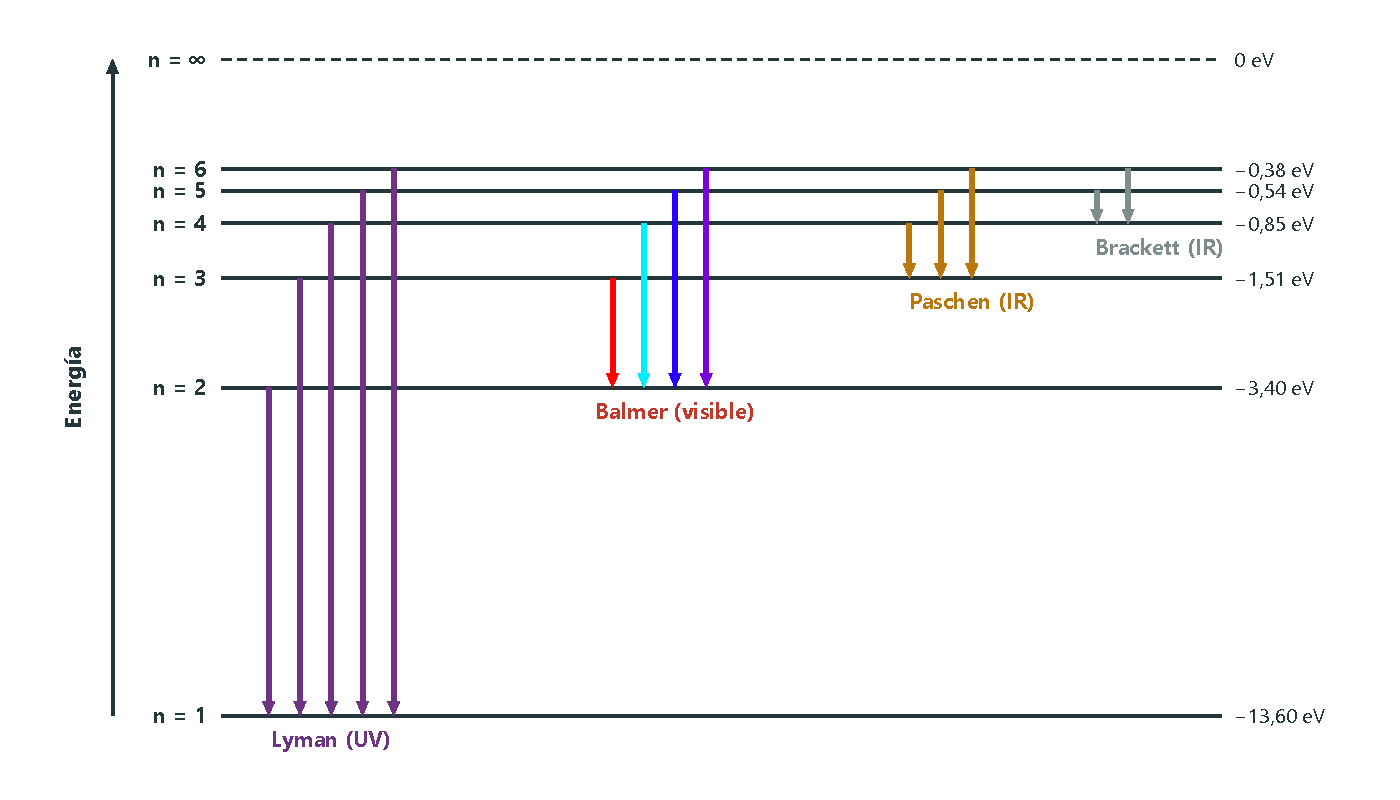
\includegraphics[width=0.8\textwidth]{images/UD3/bohr_series}
    \caption{Niveles de energía del átomo de hidrógeno y series espectrales (escala vertical comprimida para que se distingan los
    niveles altos).}
    \label{fig:ud3-series}
\end{figure}

\begin{example}
    \textbf{Niveles de energía del hidrógeno.} Calcula la energía del electrón del hidrógeno en los cinco primeros niveles.

    \textbf{Solución.} Con \(E_n = -\num{2.18e-18}/n^2\) (en julios) y \(-\num{13.6}/n^2\) (en eV):
    \begin{center}
        \begin{tabular}{@{}cccccc@{}}
            \toprule
            \(\boldsymbol{n}\) & 1 & 2 & 3 & 4 & 5 \\
            \midrule
            \(E_n\) (J) & \num{-2.18e-18} & \num{-5.45e-19} & \num{-2.42e-19} & \num{-1.36e-19} & \num{-8.72e-20} \\[3pt]
            \(E_n\) (eV) & \num{-13.6} & \num{-3.40} & \num{-1.51} & \num{-0.85} & \num{-0.54} \\
            \bottomrule
        \end{tabular}
    \end{center}
    Los niveles están cada vez más próximos entre sí a medida que aumenta \(n\).
\end{example}

\begin{example}
    \textbf{La raya roja del hidrógeno.} Calcula la energía, la frecuencia y la longitud de onda del fotón que emite el electrón
    del hidrógeno al pasar del nivel \(n = 3\) al \(n = 2\).

    \textbf{Solución.} \(\Delta E = E_3 - E_2 = \num{2.18e-18} \left( \dfrac{1}{2^2} - \dfrac{1}{3^2} \right) = \qty{3.03e-19}{\joule}\)
    es la energía del fotón emitido.
    \[ \nu = \frac{E}{h} = \frac{\num{3.03e-19}}{\num{6.626e-34}} = \qty{4.57e14}{\hertz} \qquad
    \lambda = \frac{c}{\nu} = \frac{\num{3.00e8}}{\num{4.57e14}} = \qty{6.56e-7}{\m} = \qty{656}{\nm} \]
    Es la raya roja de la serie de Balmer (figura~\ref{fig:ud3-espectros}).
\end{example}

\begin{exercise}
    a) ¿Qué energía hay que dar al electrón de un átomo de hidrógeno en su estado fundamental (\(n = 1\)) para arrancarlo del
    átomo? Exprésala en julios y en \unit{\kilo\joule\per\mol}. b) ¿Qué longitud de onda máxima debe tener la radiación capaz de
    hacerlo?
    \begin{solu}
        a) Hay que llevarlo de \(E_1\) a \(E_\infty = 0\): \(\textcolor{red}{\qty{2.18e-18}{\joule}}\) por átomo;
        \(\num{2.18e-18} \cdot \num{6.022e23} = \textcolor{red}{\qty{1313}{\kilo\joule\per\mol}}\).
        b) \(\lambda = \dfrac{h c}{E} = \textcolor{red}{\qty{9.12e-8}{\m} = \qty{91.2}{\nm}}\) (ultravioleta).
    \end{solu}
\end{exercise}

\begin{exercise}
    ¿Por qué cada elemento químico tiene un espectro diferente, que sirve para identificarlo?
    \begin{solu}
        \textcolor{red}{Porque la energía de los niveles depende de la carga del núcleo (\(Z\)) y de los demás electrones}: las
        diferencias de energía entre niveles, y por tanto las frecuencias absorbidas o emitidas, son distintas en cada elemento.
    \end{solu}
\end{exercise}

\subsection{Modificaciones al modelo de Bohr}

El modelo de Bohr no podía explicar el espectro de los átomos con más de un electrón, y los espectroscopios, cada vez mejores,
aportaban nuevos datos:
\begin{itemize}
    \item \textbf{A. Sommerfeld} observó en 1915 que algunas rayas eran en realidad dos o más rayas finas muy próximas. Propuso
    que había \textbf{subniveles} de energía y que las órbitas podían ser elípticas.
    \item El \textbf{efecto Zeeman} (1896) es el desdoblamiento de las rayas del espectro en presencia de un campo magnético. Se
    relacionó con distintas \textbf{orientaciones} de las órbitas en el espacio.
    \item \textbf{G. Uhlenbeck} y \textbf{S. Goudsmit} explicaron otro desdoblamiento de las rayas suponiendo que el electrón
    tiene \textbf{propiedades magnéticas} propias, como habían sugerido los experimentos de \textbf{O. Stern} y
    \textbf{W. Gerlach}: el \textbf{espín}.
\end{itemize}
Para describir estos cambios de subnivel, de orientación o de movimiento se introdujeron nuevos números cuánticos: \(l\),
\(m\) y \(s\). En el modelo posterior estos números surgirán de las propias ecuaciones.

\subsection{La contribución de la física cuántica}

En 1924, \textbf{L. de Broglie} propuso que, igual que la luz se comporta a veces como partícula, las partículas (como el
electrón) se comportan a veces como ondas. Poco después apareció otra idea que rompía con la física clásica:

\begin{definition}[Principio de incertidumbre de Heisenberg (1927)]
    Es imposible medir con exactitud, a la vez, la posición y la velocidad de una partícula subatómica como el electrón.
\end{definition}

Esto obliga a abandonar la idea de \textbf{órbita}, una trayectoria definida: no podemos saber a la vez dónde está el electrón y
a qué velocidad se mueve. Solo podemos hablar de la \textbf{probabilidad} de encontrarlo en una zona.

\subsection{El modelo mecanocuántico del átomo}

Había que crear leyes físicas nuevas para describir el mundo subatómico. En 1926, \textbf{E. Schrödinger} formuló una
\textbf{ecuación de onda} para estudiar el movimiento de un electrón ligado a un átomo. Sus soluciones son las
\textbf{funciones de onda}, \(\Psi\), que dependen de cuatro \textbf{números cuánticos}: \(n\), \(l\), \(m\) y \(m_s\). La función
de onda no tiene un significado físico directo, pero \(|\Psi|^2\) indica la \textbf{densidad de probabilidad} de encontrar al
electrón en cada punto (interpretación de Copenhague, de Born, Heisenberg y Bohr, a la que Einstein se opuso con su famosa frase
«Dios no juega a los dados»).

\begin{definition}[Orbital atómico]
    Es la \textbf{región del espacio} alrededor del núcleo en la que la \textbf{probabilidad} de encontrar al electrón con una
    energía determinada es máxima (superior al 90\,\%). Cada orbital queda definido por tres números cuánticos: \(n\), \(l\) y
    \(m\).
\end{definition}

\begin{remark}
    \textbf{Órbita y orbital no son lo mismo.} Una órbita (modelo de Bohr) es una trayectoria circular bien definida; un orbital
    es una «nube» de probabilidad, sin trayectoria, con una forma que depende de \(l\). En 2013 se obtuvo la primera imagen real de
    un átomo de hidrógeno: el electrón no aparece como una bolita, sino como una nube alrededor del núcleo.
\end{remark}

\subsection{Los números cuánticos}

\begin{table}[H]
    \centering
    \caption{Números cuánticos que caracterizan un orbital}
    \vspace{-5pt}
    \begin{tabular}{@{}lL{3.6cm}L{4.4cm}L{3.8cm}@{}}
        \toprule
        & \textbf{Principal, \(\boldsymbol{n}\)} & \textbf{Secundario o azimutal, \(\boldsymbol{l}\)} & \textbf{Magnético, \(\boldsymbol{m}\)} \\
        \midrule
        Valores & \(1, 2, 3\dots\) & \(0, 1, 2\dots, n-1\) & De \(-l\) a \(+l\), incluido el 0 \\[3pt]
        Indica & El \textbf{nivel} de energía & El \textbf{subnivel}: cada nivel tiene \(n\) subniveles & La \textbf{orientación} del orbital en el espacio: cada subnivel tiene \(2l+1\) orbitales \\[3pt]
        Determina & El \textbf{tamaño} del orbital & La \textbf{forma} del orbital & Su orientación \\
        \bottomrule
    \end{tabular}
    \label{tab:ud3-numeros}
\end{table}

Los subniveles se nombran con el valor de \(n\) y una letra según el valor de \(l\):
\[ l = 0 \rightarrow s \qquad l = 1 \rightarrow p \qquad l = 2 \rightarrow d \qquad l = 3 \rightarrow f \]

\begin{table}[H]
    \centering
    \caption{Subniveles y orbitales de los cuatro primeros niveles}
    \vspace{-5pt}
    \begin{tabular}{@{}cccccc@{}}
        \toprule
        \(\boldsymbol{n}\) & \(\boldsymbol{l}\) & \textbf{Subnivel} & \(\boldsymbol{m}\) & \makecell{\textbf{N.º de} \\ \textbf{orbitales}} & \makecell{\textbf{Electrones} \\ \textbf{(máximo)}} \\
        \midrule
        1 & 0 & 1s & 0 & 1 & 2 \\[3pt]
        \cmidrule(lr){1-6}
        2 & 0 & 2s & 0 & 1 & 2 \\
          & 1 & 2p & \(-1, 0, +1\) & 3 & 6 \\[3pt]
        \cmidrule(lr){1-6}
        3 & 0 & 3s & 0 & 1 & 2 \\
          & 1 & 3p & \(-1, 0, +1\) & 3 & 6 \\
          & 2 & 3d & \(-2, -1, 0, +1, +2\) & 5 & 10 \\[3pt]
        \cmidrule(lr){1-6}
        4 & 0 & 4s & 0 & 1 & 2 \\
          & 1 & 4p & \(-1, 0, +1\) & 3 & 6 \\
          & 2 & 4d & \(-2\dots +2\) & 5 & 10 \\
          & 3 & 4f & \(-3\dots +3\) & 7 & 14 \\
        \bottomrule
    \end{tabular}
    \label{tab:ud3-subniveles}
\end{table}

Los orbitales de un mismo subnivel tienen \textbf{la misma energía}. Su forma depende de \(l\) (figura~\ref{fig:ud3-orbitales}):
los \textbf{s} son esféricos; los \textbf{p}, de dos lóbulos orientados según los ejes \(x\), \(y\) o \(z\); y los \textbf{d},
más complejos, casi todos de cuatro lóbulos.

\begin{figure}[H]
    \centering
    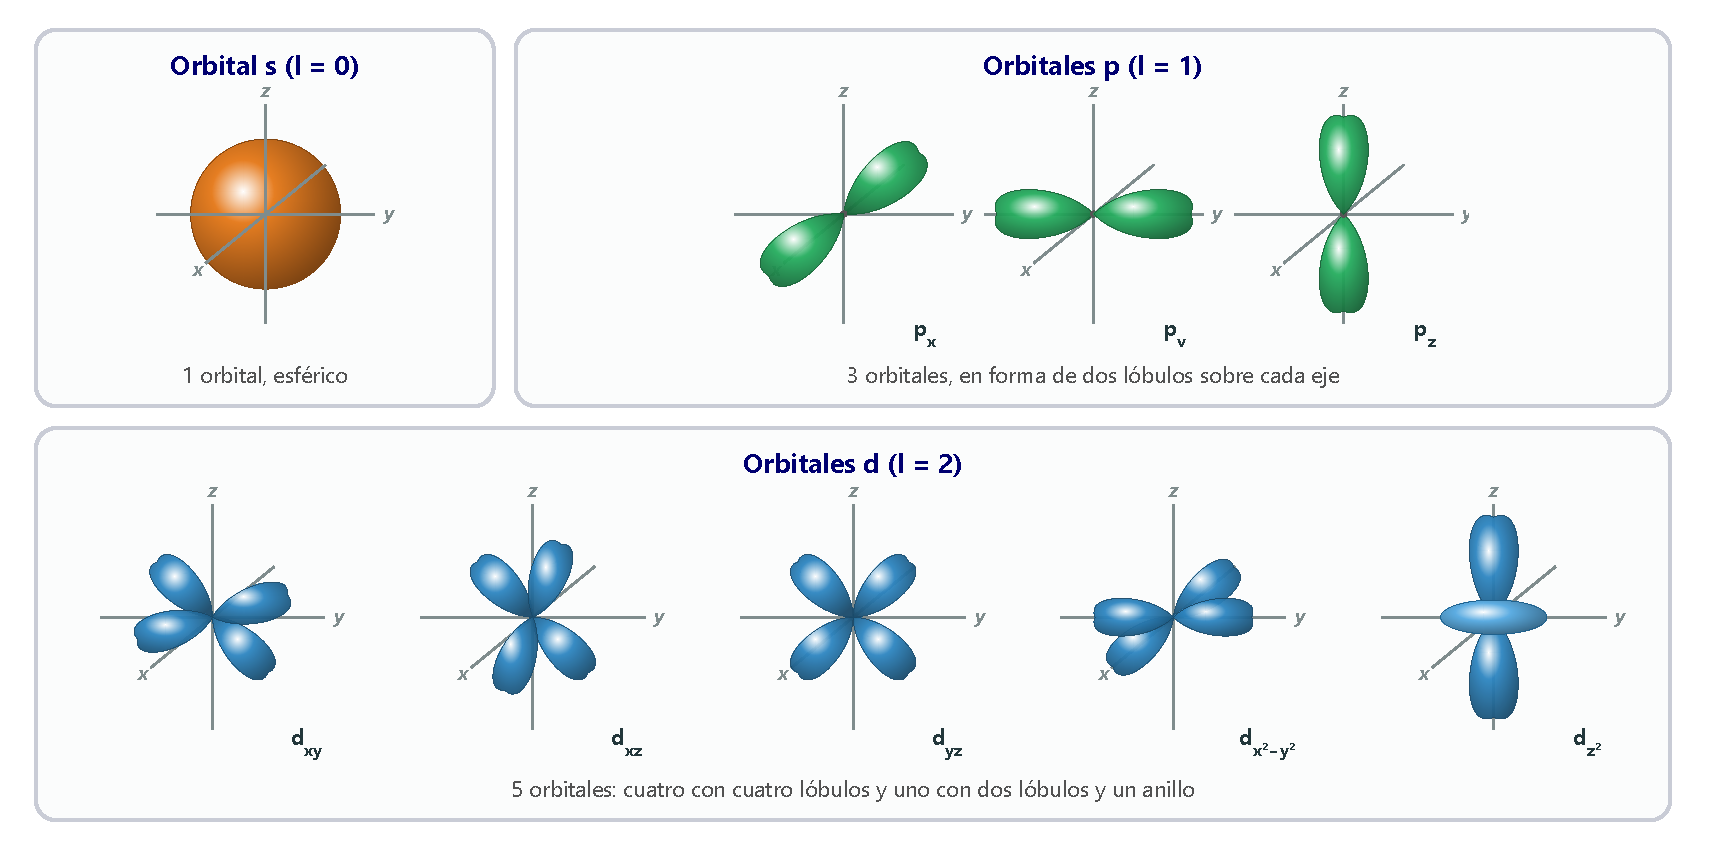
\includegraphics[width=\textwidth]{images/UD3/orbitales}
    \caption{Forma de los orbitales s, p y d.}
    \label{fig:ud3-orbitales}
\end{figure}

\paragraph{El espín del electrón.} Igual que la masa o la carga, el \textbf{espín} es una \textbf{propiedad intrínseca} de las
partículas subatómicas, relacionada con su comportamiento magnético. El \textbf{número cuántico de espín}, \(m_s\), solo puede
valer \(+\frac{1}{2}\) (se representa \(\uparrow\)) o \(-\frac{1}{2}\) (\(\downarrow\)).

El \textbf{estado} de un electrón queda determinado por sus cuatro números cuánticos \((n, l, m, m_s)\): los tres primeros
indican en qué orbital está, y \(m_s\), el sentido de su espín.

\begin{example}
    \textbf{¿Combinaciones posibles?} Indica cuáles de estos conjuntos de números cuánticos \((n, l, m, m_s)\) son posibles y, para
    los que lo sean, en qué orbital está el electrón: a) \((4, 2, -1, +\frac{1}{2})\); b) \((3, 3, 0, -\frac{1}{2})\);
    c) \((2, 1, -2, +\frac{1}{2})\).

    \textbf{Solución.} a) \textbf{Posible}: con \(n = 4\), \(l\) puede valer 0, 1, 2 o 3; con \(l = 2\), \(m\) va de \(-2\) a
    \(+2\), y \(m_s = +\frac{1}{2}\) es válido. Es un electrón de un orbital \textbf{4d}.

    b) \textbf{No es posible}: \(l\) debe ser menor que \(n\) (con \(n = 3\), \(l\) solo puede ser 0, 1 o 2).

    c) \textbf{No es posible}: con \(l = 1\), \(m\) solo puede ser \(-1\), 0 o \(+1\).
\end{example}

\begin{exercise}
    a) Para \(n = 3\), ¿qué valores pueden tomar \(l\) y \(m\)? b) ¿Cuántos orbitales hay en el nivel 3 y cuántos electrones caben
    en él? c) Generaliza: ¿cuántos orbitales y electrones hay en el nivel \(n\)?
    \begin{solu}
        a) \(l = 0\) (\(m = 0\)); \(l = 1\) (\(m = -1, 0, +1\)); \(l = 2\) (\(m = -2\dots+2\)). b) \(1 + 3 + 5 = \textcolor{red}{9}\)
        orbitales y \(\textcolor{red}{18}\) electrones. c) \(\textcolor{red}{n^2}\) orbitales y \(\textcolor{red}{2n^2}\) electrones.
    \end{solu}
\end{exercise}

\begin{exercise}
    Dados los conjuntos de números cuánticos \((4, 2, 1, -\frac{1}{2})\), \((3, 1, -2, +\frac{1}{2})\), \((2, 0, 0, +1)\) y
    \((5, 1, 0, -\frac{1}{2})\): a) ¿cuáles son posibles y por qué? b) ¿En qué orbital está el electrón en los posibles?
    c) ¿Cuál de ellos tiene más energía?
    \begin{solu}
        a) \textcolor{red}{Posibles: el primero y el cuarto.} El segundo no, porque con \(l = 1\), \(m\) no puede ser \(-2\); el
        tercero no, porque \(m_s\) solo vale \(\pm\frac{1}{2}\). b) \textcolor{red}{4d y 5p.} c) Los dos tienen \(n + l = 6\); a
        igualdad, tiene más energía el de mayor \(n\): \textcolor{red}{el 5p} (en el diagrama de Möller va después del 4d).
    \end{solu}
\end{exercise}

\subsection{Configuraciones electrónicas}

La \textbf{configuración electrónica} es la forma en que se distribuyen los electrones de un átomo en sus orbitales. La más
estable es la de menor energía, que se llama \textbf{estado fundamental}. Para escribirla se siguen tres reglas:

\begin{definition}[Reglas para escribir configuraciones electrónicas]
    \leavevmode % el título de la definición en su propia línea, la lista debajo
    \begin{enumerate}
        \item \textbf{Principio de Aufbau} (o de construcción): los electrones van ocupando los subniveles \textbf{de menor a mayor
        energía}. El orden se recuerda con el \textbf{diagrama de Möller} (figura~\ref{fig:ud3-moller}): primero se llenan los
        subniveles con menor \(n + l\), y si dos tienen el mismo, el de menor \(n\).
        \item \textbf{Principio de exclusión de Pauli}: en un átomo no puede haber dos electrones con los cuatro números cuánticos
        iguales. Como \(m_s\) solo tiene dos valores, en un orbital caben como máximo \textbf{dos electrones}, con espines
        opuestos (\(\uparrow\downarrow\)).
        \item \textbf{Regla de máxima multiplicidad de Hund}: los orbitales de un mismo subnivel se llenan de modo que haya el
        \textbf{máximo número de electrones desapareados} (con el mismo espín); solo cuando todos tienen un electrón empiezan a
        aparearse.
    \end{enumerate}
\end{definition}

\begin{figure}[H]
    \centering
    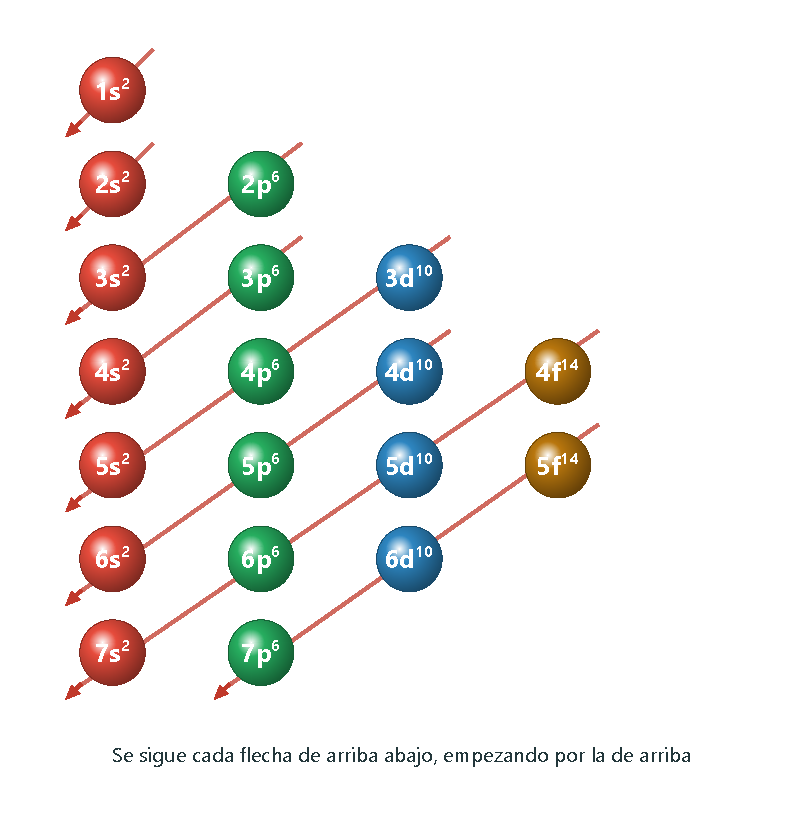
\includegraphics[width=0.45\textwidth]{images/UD3/moller}
    \caption{Diagrama de Möller: orden de llenado de los subniveles. El superíndice es el número máximo de electrones que caben
    en cada subnivel (el doble de sus orbitales).}
    \label{fig:ud3-moller}
\end{figure}

El orden de llenado es: \conf{1s\ 2s\ 2p\ 3s\ 3p\ 4s\ 3d\ 4p\ 5s\ 4d\ 5p\ 6s\ 4f\ 5d\ 6p\ 7s\ 5f\ 6d\ 7p}. Los orbitales se
representan con cajas y los electrones con flechas. Por ejemplo, así se llena un subnivel p según la regla de Hund:
\begin{center}
    \orbcaja{\uparrow}\orbcaja{}\orbcaja{}\quad \orbcaja{\uparrow}\orbcaja{\uparrow}\orbcaja{}\quad \orbcaja{\uparrow}\orbcaja{\uparrow}\orbcaja{\uparrow}\quad
    \orbcaja{\uparrow\downarrow}\orbcaja{\uparrow}\orbcaja{\uparrow}\quad \orbcaja{\uparrow\downarrow}\orbcaja{\uparrow\downarrow}\orbcaja{\uparrow}\quad
    \orbcaja{\uparrow\downarrow}\orbcaja{\uparrow\downarrow}\orbcaja{\uparrow\downarrow}
\end{center}
Un orbital puede estar \textbf{vacío}, \textbf{semilleno} (un electrón desapareado) o \textbf{lleno} (dos electrones apareados).

\paragraph{Átomos e iones.}
\begin{itemize}
    \item Un átomo \textbf{neutro} tiene \(Z\) electrones: el aluminio (\(Z = 13\)) tiene 13: \conf{1s^2\,2s^2\,2p^6\,3s^2\,3p^1}.
    \item Un \textbf{catión} tiene tantos electrones menos como indica su carga: el \ch{Al^3+} tiene \(13 - 3 = 10\) electrones:
    \conf{1s^2\,2s^2\,2p^6}.
    \item Un \textbf{anión} tiene tantos electrones más como indica su carga: el \ch{S^2-} tiene \(16 + 2 = 18\) electrones:
    \conf{1s^2\,2s^2\,2p^6\,3s^2\,3p^6}.
\end{itemize}

\begin{remark}
    \textbf{Los metales de transición pierden primero los electrones 4s.} Aunque el 4s se llena antes que el 3d, una vez ocupado
    el 3d su energía queda por debajo de la del 4s. Por eso, al formar cationes, los metales de transición pierden primero los
    electrones del nivel más externo: \ch{Fe} \conf{[Ar]\,4s^2\,3d^6} \(\rightarrow\) \ch{Fe^2+} \conf{[Ar]\,3d^6}. Hay
    además algunas excepciones a las reglas de llenado, como el cromo (\conf{[Ar]\,4s^1\,3d^5}) y el cobre
    (\conf{[Ar]\,4s^1\,3d^{10}}), que se estabilizan con subniveles d semillenos o llenos.
\end{remark}

\begin{example}
    \textbf{Configuraciones electrónicas.} Escribe la configuración electrónica de: a) N (\(Z = 7\)); b) \ch{Cl^-} (\(Z = 17\));
    c) \ch{Fe^2+} (\(Z = 26\)); d) Br (\(Z = 35\)).

    \textbf{Solución.} Seguimos el orden del diagrama de Möller:

    a) N (7 electrones): \conf{1s^2\,2s^2\,2p^3}.

    b) Cl (17 electrones): \conf{1s^2\,2s^2\,2p^6\,3s^2\,3p^5}.\\
    Al ganar un electrón, \ch{Cl^-} (18 electrones): \conf{1s^2\,2s^2\,2p^6\,3s^2\,3p^6}.

    c) Fe (26 electrones): \conf{1s^2\,2s^2\,2p^6\,3s^2\,3p^6\,4s^2\,3d^6}.\\
    Pierde los dos electrones 4s: \ch{Fe^2+} \conf{1s^2\,2s^2\,2p^6\,3s^2\,3p^6\,3d^6}.

    d) Br (35 electrones): \conf{1s^2\,2s^2\,2p^6\,3s^2\,3p^6\,4s^2\,3d^{10}\,4p^5}.
\end{example}

\begin{example}
    \textbf{¿Estado fundamental o excitado?} ¿Alguna de estas configuraciones corresponde a un átomo en estado excitado?
    a) \conf{1s^2\,2s^2\,2p^6\,3s^2\,3p^4\,4s^1}; b) \conf{1s^2\,2s^2\,2p^6\,3s^2\,3p^6\,4s^2\,3d^3}; c) \conf{1s^2\,2s^2\,2p^4\,3s^1}.

    \textbf{Solución.} a) Tiene 17 electrones; en el estado fundamental el 3p estaría completo (\(3p^5\)) antes de ocupar el 4s:
    es el cloro en un \textbf{estado excitado}. b) Tiene 23 electrones colocados en orden: es el vanadio en su \textbf{estado
    fundamental}. c) Tiene 9 electrones y el 2p no está completo: es el flúor \textbf{excitado} (el fundamental es
    \conf{1s^2\,2s^2\,2p^5}).
\end{example}

\begin{exercise}
    Para el isótopo \ch{^{85}_{37}Rb}, indica: a) el número de protones, neutrones y electrones; b) su configuración electrónica y
    el número de electrones desapareados; c) los números cuánticos de su último electrón; d) el ion más estable que puede formar.
    \begin{solu}
        a) \textcolor{red}{37 p, 48 n y 37 e}. b) \(\textcolor{red}{\conf{1s^2\,2s^2\,2p^6\,3s^2\,3p^6\,4s^2\,3d^{10}\,4p^6\,5s^1}}\);
        \textcolor{red}{un electrón desapareado}. c) \(\textcolor{red}{(5, 0, 0, +\frac{1}{2})}\). d) \textcolor{red}{\ch{Rb^+}}:
        al perder el electrón 5s queda con la configuración del criptón.
    \end{solu}
\end{exercise}

\begin{exercise}
    Ordena de menor a mayor energía los subniveles 3d, 4s, 2p, 5s y 4p, y escribe un conjunto posible de números cuánticos para
    un electrón de cada uno.
    \begin{solu}
        \textcolor{red}{2p \(<\) 4s \(<\) 3d \(<\) 4p \(<\) 5s} (\(n + l\) = 3, 4, 5, 5, 5; a igual \(n + l\), menor \(n\)).
        Por ejemplo: 2p \((2, 1, 0, +\frac{1}{2})\); 4s \((4, 0, 0, -\frac{1}{2})\); 3d \((3, 2, -2, +\frac{1}{2})\);
        4p \((4, 1, 1, +\frac{1}{2})\); 5s \((5, 0, 0, +\frac{1}{2})\).
    \end{solu}
\end{exercise}

\begin{exercise}
    Escribe el diagrama de orbitales (cajas) de la última capa del nitrógeno (\(Z = 7\)) y del oxígeno (\(Z = 8\)), y del subnivel
    3d del hierro (\(Z = 26\)). ¿Cuántos electrones desapareados tiene cada uno?
    \begin{solu}
        N: 2s \orbcaja{\uparrow\downarrow} 2p \orbcaja{\uparrow}\orbcaja{\uparrow}\orbcaja{\uparrow}: \textcolor{red}{3 desapareados}.
        O: 2s \orbcaja{\uparrow\downarrow} 2p \orbcaja{\uparrow\downarrow}\orbcaja{\uparrow}\orbcaja{\uparrow}: \textcolor{red}{2}.
        Fe: 3d \orbcaja{\uparrow\downarrow}\orbcaja{\uparrow}\orbcaja{\uparrow}\orbcaja{\uparrow}\orbcaja{\uparrow}: \textcolor{red}{4}.
    \end{solu}
\end{exercise}

%========================================================================================
\section{La clasificación periódica de los elementos}\label{sec:ud3-tabla}
%========================================================================================

El oro, la plata o el cobre se conocen desde la Antigüedad, pero fue en el siglo XVIII cuando empezaron a aislarse elementos en
el laboratorio. En el siglo XIX, la electrólisis y la espectroscopía permitieron descubrir muchos más: en 1830 se conocían 55. El
estudio de la radiactividad, en el siglo XX, elevó la cifra hasta los \textbf{118} elementos actuales, de los cuales una veintena
se han sintetizado en aceleradores de partículas o reactores nucleares y no se han encontrado en la naturaleza.

\subsection{Clasificando los elementos a lo largo de la historia}

Pronto se vio que algunos elementos tenían propiedades químicas y físicas parecidas. ¿Qué criterio permitiría clasificarlos?
\begin{itemize}
    \item \textbf{J.\,W. Döbereiner} (1780-1849) formó grupos de tres elementos parecidos, ordenados por masa atómica, las
    \textbf{tríadas}: cloro, bromo y yodo; azufre, selenio y teluro.
    \item \textbf{A. de Chancourtois} (1862) colocó los elementos en una espiral sobre un cilindro y descubrió la
    \textbf{periodicidad}: las propiedades se repetían a intervalos regulares.
    \item \textbf{J. Newlands} ordenó los elementos por su masa en \textbf{octavas}: el octavo se parecía al primero, como las
    notas musicales.
    \item \textbf{D. Mendeléiev} (1869) y, poco después, \textbf{L. Meyer} ordenaron los elementos por su masa atómica en una
    \textbf{tabla}, de forma que en la misma columna quedaran los elementos de propiedades semejantes. Mendeléiev dejó
    \textbf{huecos} para elementos aún desconocidos, cuyas propiedades predijo con acierto (como el galio o el germanio), y
    cambió de orden algunos elementos para que quedaran en la familia que les correspondía por sus propiedades.
    \item \textbf{H. Moseley} (1913) midió la carga nuclear de los átomos y demostró que el número atómico \(Z\) es característico
    de cada elemento. Ordenándolos por \(Z\) y no por su masa, cada elemento encajaba en su familia de forma natural.
\end{itemize}

\begin{remark}
    \textbf{Mujeres y elementos.} Marie Skłodowska-Curie descubrió el polonio y el radio, y el curio lleva su nombre y el de su
    marido; Lise Meitner encontró un isótopo del protactinio, y el meitnerio se llama así en su honor; Ida Noddack descubrió el
    renio, y Marguerite Perey, el francio.
\end{remark}

\subsection{La tabla periódica actual}

A partir de la propuesta de Mendeléiev y de las aportaciones posteriores se llegó a la tabla actual
(figura~\ref{fig:ud3-tabla}). Los elementos están ordenados por su número atómico en \textbf{7 filas o periodos} y
\textbf{18 columnas o grupos}, numerados del 1 al 18. Los elementos de un mismo grupo tienen propiedades semejantes y forman una
\textbf{familia}. Los periodos 6 y 7 tienen 14 elementos más cada uno, que se colocan aparte, debajo de la tabla, para que no
quede demasiado ancha.

\begin{figure}[H]
    \centering
    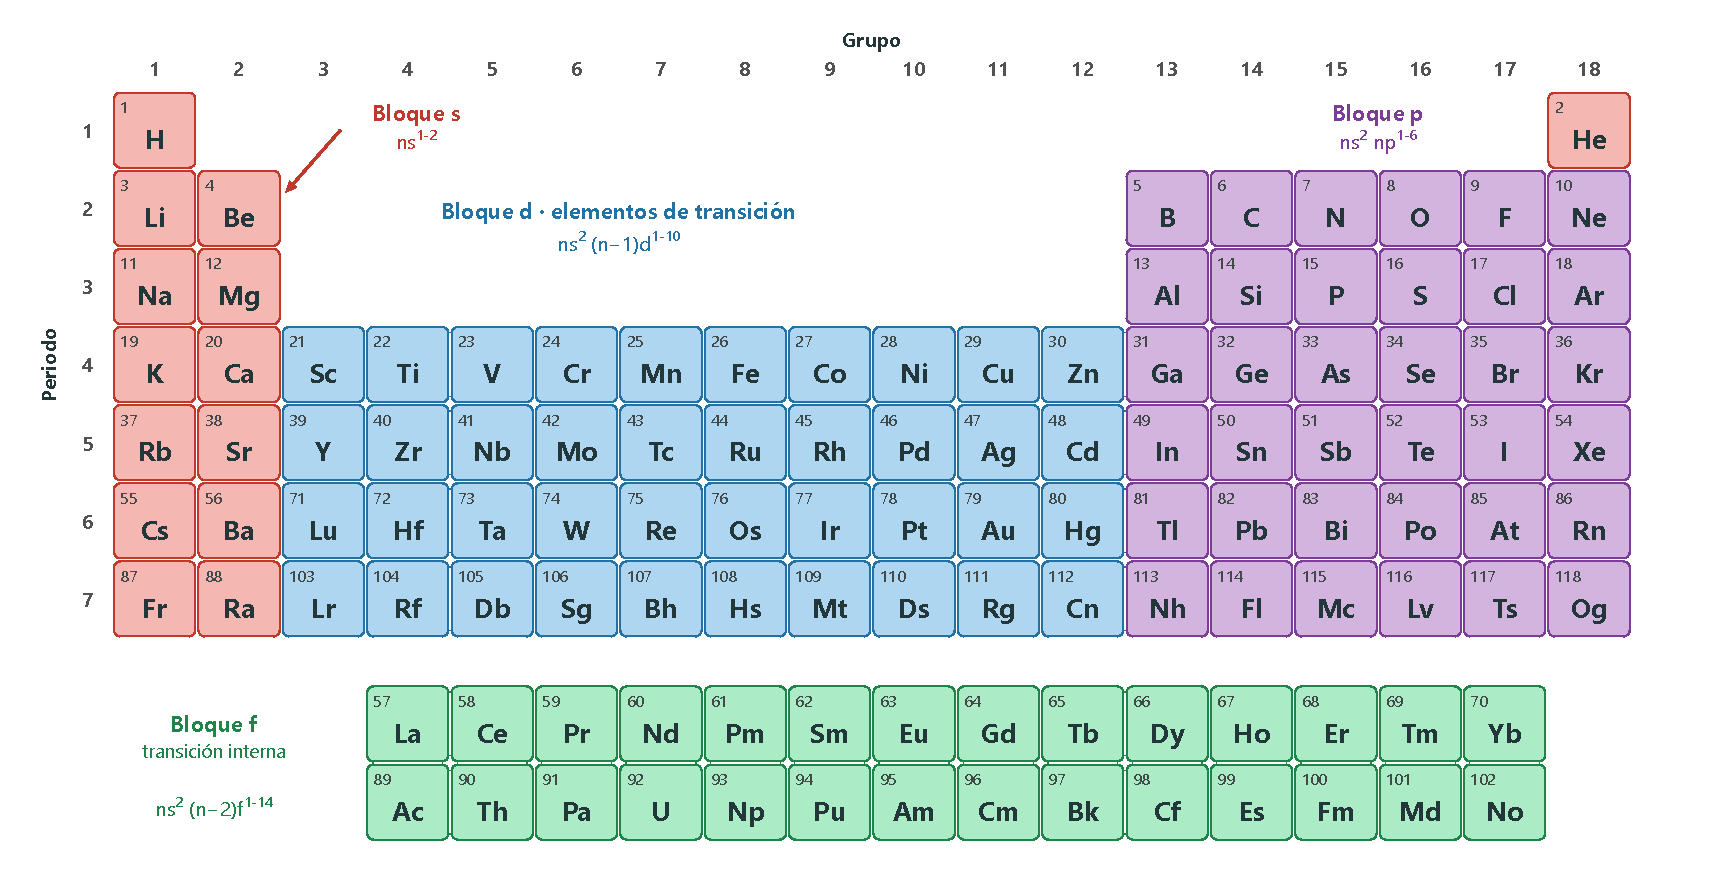
\includegraphics[width=\textwidth]{images/UD3/tabla_bloques}
    \caption{Tabla periódica actual, con los bloques s, p, d y f.}
    \label{fig:ud3-tabla}
\end{figure}

\subsection{Tabla periódica y configuración electrónica}

¿Por qué el berilio (\(Z = 4\)) y el bario (\(Z = 56\)) se parecen? ¿Por qué las propiedades se repiten a intervalos regulares?
Bohr fue el primero en relacionar la configuración electrónica con la posición en la tabla. Fíjate en los elementos del grupo 1:
\begin{center}
    Li \conf{1s^2\,2s^1} \qquad Na \conf{1s^2\,2s^2\,2p^6\,3s^1} \qquad K \conf{[Ne]\,3s^2\,3p^6\,4s^1} \qquad Rb \conf{[Ar]\,4s^2\,3d^{10}\,4p^6\,5s^1}
\end{center}
Todos tienen \textbf{un solo electrón} en el orbital s del último nivel: su configuración termina en \conf{ns^1}.

\begin{definition}[Capa de valencia]
    Es el último nivel (el más externo) en el que hay electrones. Sus electrones se llaman \textbf{electrones de valencia}, y son
    los que determinan las propiedades químicas del elemento.
\end{definition}

\begin{remark}
    Para abreviar, la configuración se escribe a menudo a partir de la del \textbf{gas noble anterior}, entre corchetes:
    Fe \conf{1s^2\,2s^2\,2p^6\,3s^2\,3p^6\,4s^2\,3d^6} = \conf{[Ar]\,4s^2\,3d^6}.
\end{remark}

\begin{itemize}
    \item Los elementos de un \textbf{grupo} tienen el mismo número de electrones en la última capa, en orbitales del mismo tipo.
    \item El valor más alto de \(n\) de la configuración indica el \textbf{periodo}.
    \item Según el último subnivel que se llena, la tabla se divide en \textbf{bloques} (figura~\ref{fig:ud3-tabla}):
    \begin{itemize}
        \item \textbf{Bloque s} (grupos 1 y 2): terminan en \conf{ns^1} o \conf{ns^2}.
        \item \textbf{Bloque p} (grupos 13 a 18): terminan en \conf{ns^2\,np^1} a \conf{ns^2\,np^6}. El \textbf{helio},
        \conf{1s^2}, se coloca en el grupo 18 porque, como los demás \textbf{gases nobles}, tiene su última capa completa.
        \item \textbf{Bloque d} (grupos 3 a 12), los \textbf{metales de transición}: sus últimos electrones van a orbitales d del
        \textbf{penúltimo} nivel, \(n - 1\). El hierro, por ejemplo, termina en \conf{4s^2\,3d^6}.
        \item \textbf{Bloque f}, los elementos de \textbf{transición interna} (lantánidos y actínidos), en dos filas de 14
        elementos de los periodos 6 y 7: sus últimos electrones van a orbitales f del \textbf{antepenúltimo} nivel, \(n - 2\).
        El uranio, por ejemplo, es \conf{[Rn]\,7s^2\,5f^4} (en realidad, \conf{[Rn]\,7s^2\,5f^3\,6d^1}).
    \end{itemize}
\end{itemize}

\begin{remark}
    La configuración electrónica de un elemento determina sus propiedades físicas y químicas. Por eso los elementos de un mismo
    grupo, con la misma configuración de la capa de valencia, se parecen tanto.
\end{remark}

\begin{example}
    \textbf{Elementos del mismo grupo.} Escribe la configuración de tres elementos del grupo 2 y de tres del grupo 17. ¿Qué
    tienen en común los de cada grupo?

    \textbf{Solución.} Grupo 2: Be \conf{1s^2\,2s^2}; Mg \conf{1s^2\,2s^2\,2p^6\,3s^2}; Ca \conf{1s^2\,2s^2\,2p^6\,3s^2\,3p^6\,4s^2}.
    Grupo 17: F \conf{1s^2\,2s^2\,2p^5}; Cl \conf{1s^2\,2s^2\,2p^6\,3s^2\,3p^5}; Br \conf{[Ar]\,4s^2\,3d^{10}\,4p^5}.

    Los del grupo 2 tienen una capa de valencia \conf{ns^2}, con 2 electrones de valencia; los del grupo 17, \conf{ns^2\,np^5},
    con 7 electrones de valencia.
\end{example}

\begin{example}
    \textbf{Posición en la tabla.} Escribe la configuración electrónica de O (\(Z = 8\)), Na (\(Z = 11\)), Si (\(Z = 14\)) y
    Ca (\(Z = 20\)) y, a partir de ella, indica su grupo y su periodo.

    \textbf{Solución.} O \conf{1s^2\,2s^2\,2p^4}: termina en \conf{ns^2\,np^4} con \(n = 2\): grupo 16, periodo 2.
    Na \conf{1s^2\,2s^2\,2p^6\,3s^1}: \conf{ns^1}, grupo 1, periodo 3. Si \conf{1s^2\,2s^2\,2p^6\,3s^2\,3p^2}: \conf{ns^2\,np^2},
    grupo 14, periodo 3. Ca \conf{[Ar]\,4s^2}: \conf{ns^2}, grupo 2, periodo 4.
\end{example}

\begin{exercise}
    Un elemento está en el periodo 4 y en el grupo 15. a) Escribe su configuración electrónica. b) ¿Cuál es su número atómico y de
    qué elemento se trata? c) ¿Cuántos electrones desapareados tiene?
    \begin{solu}
        a) Termina en \conf{4s^2\,4p^3}: \(\textcolor{red}{\conf{1s^2\,2s^2\,2p^6\,3s^2\,3p^6\,4s^2\,3d^{10}\,4p^3}}\).
        b) \(\textcolor{red}{Z = 33}\): \textcolor{red}{arsénico}. c) \textcolor{red}{3} (uno en cada orbital 4p).
    \end{solu}
\end{exercise}

%========================================================================================
\subsection{Propiedades periódicas}
%========================================================================================

Hay propiedades que dependen de la configuración electrónica y que, por tanto, \textbf{varían de forma periódica} a lo largo de
la tabla. Para entenderlas hay que pensar en las fuerzas que actúan sobre los electrones de la capa de valencia. Las cargas
eléctricas se atraen si son de signo contrario y se repelen si son del mismo signo, con una fuerza que, según la
\textbf{ley de Coulomb}, es
\[ F = K \frac{q \cdot q'}{r^2} \]
mayor cuanto mayores son las cargas y menor la distancia que las separa. Así:
\begin{itemize}
    \item Cada electrón es \textbf{atraído} por el núcleo, cuya carga es \(Z\) veces la carga elemental: la atracción aumenta con
    \(Z\) y disminuye con la distancia al núcleo.
    \item A la vez, cada electrón es \textbf{repelido} por los demás electrones: la atracción del núcleo sobre los electrones
    externos queda \textbf{apantallada} por los electrones de las capas internas. La carga que «sienten» de verdad los
    electrones de valencia es la \textbf{carga nuclear efectiva}.
\end{itemize}

\paragraph{Radio atómico.}

\begin{definition}[Radio atómico]
    Es la distancia del núcleo al electrón más externo. Como el átomo no tiene un borde definido, se calcula como la mitad de la
    distancia entre los núcleos de dos átomos iguales unidos.
\end{definition}

\begin{itemize}
    \item En un \textbf{grupo}, el radio \textbf{aumenta hacia abajo}: cada elemento tiene una capa electrónica más que el
    anterior. Por ejemplo, Li \qty{152}{\pico\metre}, Na \qty{186}{\pico\metre}, K \qty{227}{\pico\metre}, Rb
    \qty{248}{\pico\metre}, Cs \qty{265}{\pico\metre}.
    \item En un \textbf{periodo}, el radio \textbf{disminuye hacia la derecha}: los electrones se colocan en la misma capa, pero
    la carga nuclear efectiva aumenta y los atrae con más fuerza. Por ejemplo, en el periodo 2: Li 152, Be 112, B 88, C 77,
    N 75, O 73, F \qty{72}{\pico\metre}.
\end{itemize}

\begin{figure}[H]
    \centering
    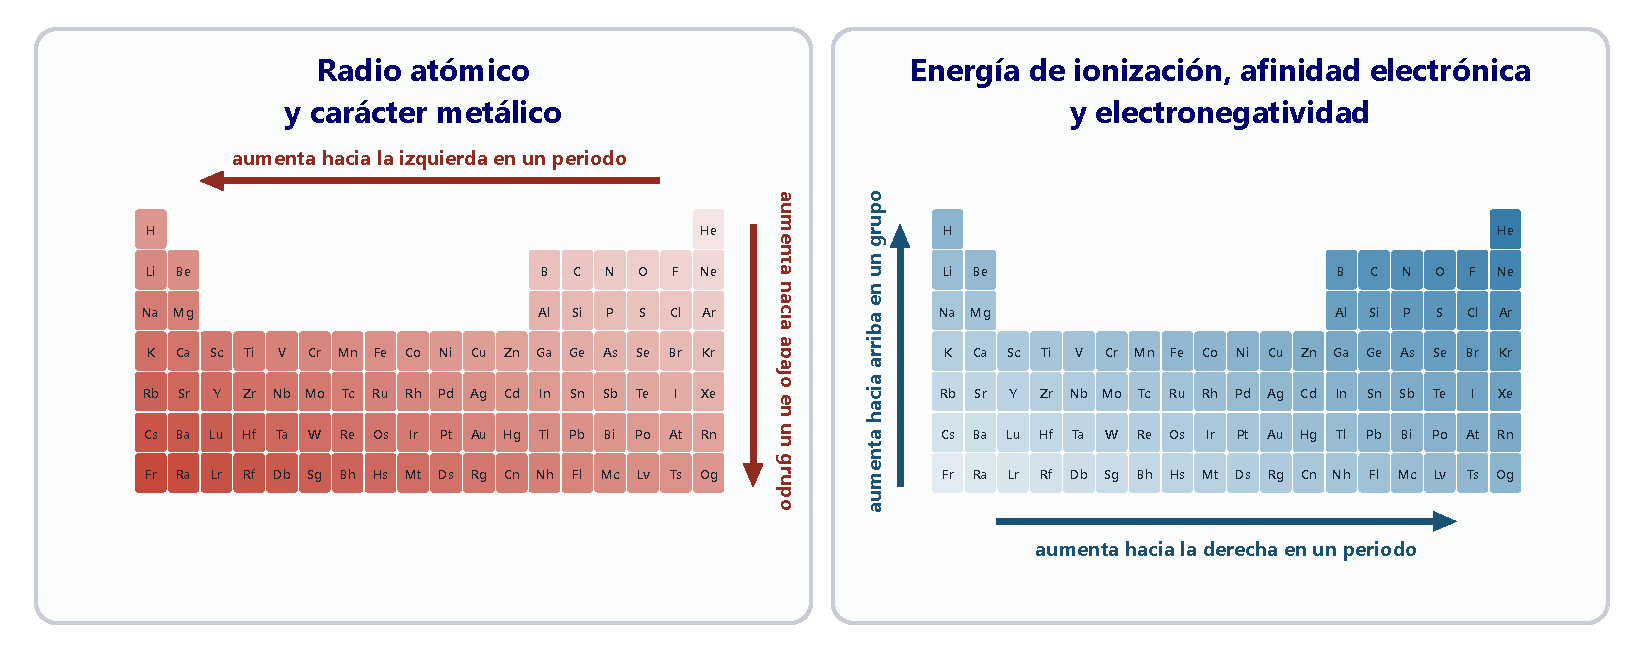
\includegraphics[width=\textwidth]{images/UD3/tendencias}
    \caption{Variación de las propiedades periódicas (cuanto más oscuro, mayor es el valor).}
    \label{fig:ud3-tendencias}
\end{figure}

\paragraph{Radio iónico.} El tamaño de un ion es distinto del de su átomo neutro (figura~\ref{fig:ud3-radios}):
\begin{itemize}
    \item Un \textbf{catión} es \textbf{más pequeño} que su átomo: suele perder la capa más externa y los electrones restantes son
    atraídos con más fuerza por el mismo número de protones.
    \item Un \textbf{anión} es \textbf{más grande} que su átomo: el electrón ganado aumenta la repulsión entre electrones y el
    apantallamiento, y la nube electrónica se expande.
\end{itemize}

\begin{figure}[H]
    \centering
    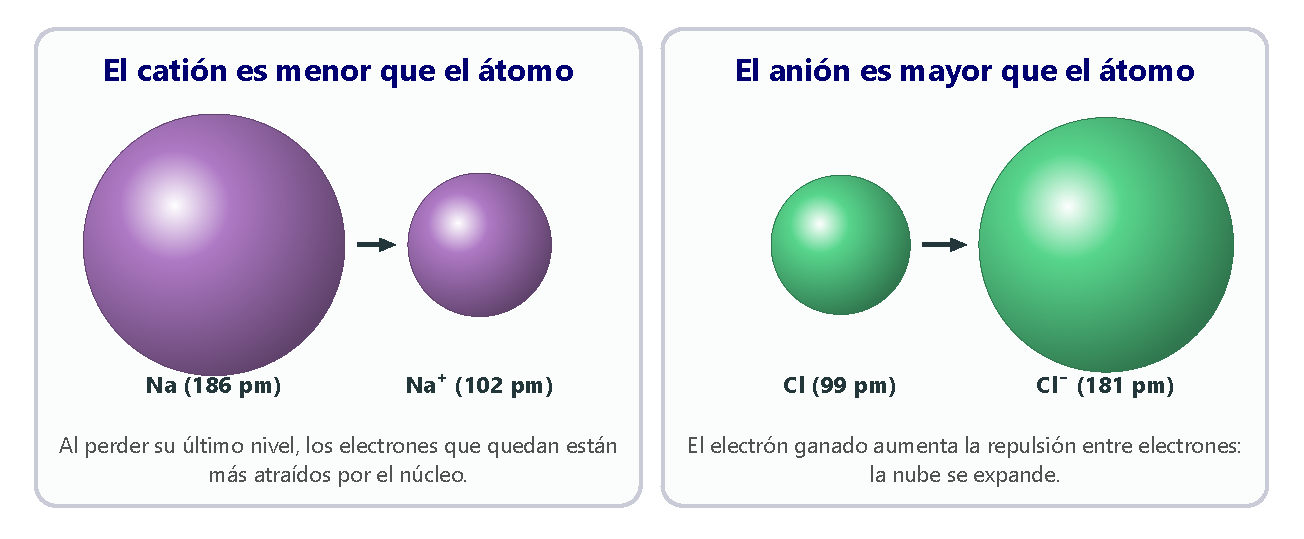
\includegraphics[width=0.75\textwidth]{images/UD3/radios_ionicos}
    \caption{Radios de los átomos de sodio y cloro y de sus iones.}
    \label{fig:ud3-radios}
\end{figure}

\begin{example}
    \textbf{Ordenar por radio atómico.} Ordena de menor a mayor radio atómico: a) Be, Mg, Ca, Sr; b) K, Ca, Ga, Br.

    \textbf{Solución.} a) Son del grupo 2: el radio aumenta al bajar en el grupo, porque hay más capas:
    \(\mathrm{Be} < \mathrm{Mg} < \mathrm{Ca} < \mathrm{Sr}\).

    b) Son del periodo 4: el radio disminuye hacia la derecha, porque aumenta la carga nuclear efectiva:
    \(\mathrm{Br} < \mathrm{Ga} < \mathrm{Ca} < \mathrm{K}\).
\end{example}

\paragraph{Energía de ionización.}

\begin{definition}[Energía de ionización]
    Es la energía necesaria para \textbf{arrancar el electrón más externo} de un átomo en estado gaseoso y fundamental,
    convirtiéndolo en un ion positivo:
    \[ \ch{X(g)} + \text{energía de ionización} \rightarrow \ch{X^+(g) + e^-} \]
    Se suele dar en \unit{\kilo\joule\per\mol}: la energía necesaria para ionizar un mol de átomos. También se usa el
    \textbf{electronvolt} por átomo: \(\qty{1}{\electronvolt} = \qty{1.602e-19}{\joule}\), y
    \(\qty{1}{\electronvolt}/\text{átomo} =\qty{96.49}{\kilo\joule\per\mol}\).
\end{definition}

Cuanto más alejado del núcleo esté el electrón, más débilmente unido está y más fácil es arrancarlo. Por eso la energía de
ionización varía al revés que el radio atómico:
\begin{itemize}
    \item En un \textbf{grupo}, \textbf{aumenta hacia arriba}: Cs 376, Rb 403, K 419, Na 496, Li \qty{520}{\kilo\joule\per\mol}.
    \item En un \textbf{periodo}, \textbf{aumenta hacia la derecha}, y es máxima en los gases nobles (figura~\ref{fig:ud3-ei}).
\end{itemize}

\begin{figure}[H]
    \centering
    \begin{tikzpicture}
        \begin{axis}[grafica, width=0.85\linewidth, height=5.5cm, xmin=0, xmax=21, ymin=0, ymax=2600,
            xtick={1,...,20}, xticklabels={H,He,Li,Be,B,C,N,O,F,Ne,Na,Mg,Al,Si,P,S,Cl,Ar,K,Ca},
            xlabel={Elemento}, ylabel={\(E_i\) (kJ/mol)}, x tick label style={font=\scriptsize},
            y tick label style={/pgf/number format/1000 sep={}}]
            \addplot[ocre, thick, mark=*, mark size=1.6pt] coordinates {(1,1312) (2,2372) (3,520) (4,900) (5,801) (6,1086) (7,1402)
                (8,1314) (9,1681) (10,2081) (11,496) (12,738) (13,578) (14,787) (15,1012) (16,1000) (17,1251) (18,1521) (19,419) (20,590)};
            \node[font=\scriptsize, anchor=south] at (axis cs:2,2372) {gases nobles};
            \node[font=\scriptsize, anchor=north] at (axis cs:11,450) {alcalinos};
        \end{axis}
    \end{tikzpicture}
    \caption{Primera energía de ionización de los 20 primeros elementos: máximos en los gases nobles y mínimos en los alcalinos.}
    \label{fig:ud3-ei}
\end{figure}

\begin{remark}
    \textbf{Energías de ionización sucesivas.} La \textbf{segunda energía de ionización} es la necesaria para arrancar un segundo
    electrón al ion \ch{X^+}, y así sucesivamente. Cada una es mayor que la anterior, porque se arranca un electrón a un ion
    cada vez más positivo, pero el aumento no es uniforme: se dispara cuando el electrón sale de una capa completa. Para el
    magnesio, \conf{[Ne]\,3s^2}:
    \[ E_{i,1} = \qty{738}{\kilo\joule\per\mol} \qquad E_{i,2} = \qty{1451}{\kilo\joule\per\mol} \qquad E_{i,3} = \qty{7733}{\kilo\joule\per\mol} \]
    El tercer electrón hay que sacarlo del nivel 2, completo y mucho más cercano al núcleo. Por eso el magnesio forma iones
    \ch{Mg^2+} y no \ch{Mg^3+}.
\end{remark}

\begin{example}
    \textbf{Ordenar por energía de ionización.} Ordena de menor a mayor primera energía de ionización: a) Li, Na, K, Cs;
    b) Na, Si, P, Cl.

    \textbf{Solución.} a) Son del grupo 1: la energía de ionización aumenta al subir en el grupo:
    \(\mathrm{Cs} < \mathrm{K} < \mathrm{Na} < \mathrm{Li}\).

    b) Son del periodo 3: aumenta hacia la derecha: \(\mathrm{Na} < \mathrm{Si} < \mathrm{P} < \mathrm{Cl}\) (los valores reales
    son 496, 787, 1012 y \qty{1251}{\kilo\joule\per\mol}).
\end{example}

\paragraph{Afinidad electrónica.} Es la energía que se intercambia cuando un átomo en estado gaseoso y fundamental
\textbf{capta un electrón} y se convierte en un ion negativo: \(\ch{X(g) + e^-} \rightarrow \ch{X^-(g)}\). Normalmente se
desprende energía (por eso suele tener signo negativo), y cuanta más se desprende, mayor es la tendencia del átomo a captar
electrones. La afinidad electrónica es mayor (en valor absoluto) \textbf{hacia arriba en un grupo} y \textbf{hacia la derecha en
un periodo}, sin contar los gases nobles: el cloro (\qty{-349}{\kilo\joule\per\mol}) y el flúor
(\qty{-328}{\kilo\joule\per\mol}) son los que más energía desprenden.

\paragraph{Electronegatividad.}

\begin{definition}[Electronegatividad]
    Es una medida de la \textbf{tendencia} de un átomo a \textbf{atraer} hacia sí los electrones del enlace que comparte con otro
    átomo.
\end{definition}

Los valores de electronegatividad se asignan \textbf{comparando} unos elementos con otros. En la escala de \textbf{Pauling}, el
más electronegativo, el flúor, tiene un 4,0. La electronegatividad \textbf{aumenta hacia arriba en un grupo} y \textbf{hacia la
derecha en un periodo} (los gases nobles, que casi no forman enlaces, no tienen valor asignado).

\begin{table}[H]
    \centering
    \caption{Electronegatividad de Pauling de los elementos representativos}
    \vspace{-5pt}
    \begin{tabular}{@{}lccccccc@{}}
        \toprule
        \textbf{Periodo} & \textbf{G. 1} & \textbf{G. 2} & \textbf{G. 13} & \textbf{G. 14} & \textbf{G. 15} & \textbf{G. 16} & \textbf{G. 17} \\
        \midrule
        1 & H 2,2 & & & & & & \\[3pt]
        2 & Li 1,0 & Be 1,6 & B 2,0 & C 2,6 & N 3,0 & O 3,4 & F 4,0 \\[3pt]
        3 & Na 0,9 & Mg 1,3 & Al 1,6 & Si 1,9 & P 2,2 & S 2,6 & Cl 3,2 \\[3pt]
        4 & K 0,8 & Ca 1,0 & Ga 1,8 & Ge 2,0 & As 2,2 & Se 2,6 & Br 3,0 \\[3pt]
        5 & Rb 0,8 & Sr 1,0 & In 1,8 & Sn 2,0 & Sb 2,1 & Te 2,1 & I 2,7 \\[3pt]
        6 & Cs 0,8 & Ba 0,9 & Tl 1,6 & Pb 2,3 & Bi 2,0 & Po 2,0 & At 2,2 \\
        \bottomrule
    \end{tabular}
    \label{tab:ud3-en}
\end{table}

\paragraph{Carácter metálico.} Los \textbf{metales} tienden a perder electrones y formar cationes: tienen energía de ionización
y electronegatividad bajas. Cuanto menor es la electronegatividad de un elemento, mayor es su \textbf{carácter metálico}, que
aumenta \textbf{hacia abajo y hacia la izquierda} de la tabla. Los \textbf{no metales}, a la derecha y arriba, tienden a captar
electrones y formar aniones.

\begin{example}
    \textbf{Ordenar por electronegatividad.} Ordena de menor a mayor electronegatividad: Rb, Ti, As, O y F.

    \textbf{Solución.} La electronegatividad aumenta hacia arriba y hacia la derecha. El Rb (grupo 1, periodo 5) es el que está
    más abajo y a la izquierda, y el F, el que está más arriba y a la derecha. El Ti y el As están en el periodo 4, el Ti más a
    la izquierda; el O está en el periodo 2:
    \(\mathrm{Rb} < \mathrm{Ti} < \mathrm{As} < \mathrm{O} < \mathrm{F}\) (0,8; 1,5; 2,2; 3,4 y 4,0).
\end{example}

\begin{exercise}
    Para la pareja de elementos K y Br, razona: a) cuál tiene mayor radio; b) cuál tiene mayor energía de ionización; c) cuál es
    más electronegativo.
    \begin{solu}
        Los dos están en el periodo 4; el K en el grupo 1 y el Br en el 17. a) \textcolor{red}{El K}: el radio disminuye hacia la
        derecha. b) \textcolor{red}{El Br}: la energía de ionización aumenta hacia la derecha. c) \textcolor{red}{El Br}.
    \end{solu}
\end{exercise}

\begin{exercise}
    Para los elementos A (\(Z = 17\)) y B (\(Z = 20\)): a) escribe sus configuraciones electrónicas; b) indica el ion más estable de
    cada uno; c) ¿cuál de los dos iones tiene mayor radio?
    \begin{solu}
        a) A: \conf{1s^2\,2s^2\,2p^6\,3s^2\,3p^5} (cloro); B: \conf{1s^2\,2s^2\,2p^6\,3s^2\,3p^6\,4s^2} (calcio).
        b) \textcolor{red}{\ch{A^-} (\ch{Cl^-}) y \ch{B^2+} (\ch{Ca^2+})}: ambos adquieren la configuración del argón.
        c) Los dos iones tienen 18 electrones, pero el \ch{Cl^-} solo 17 protones frente a los 20 del \ch{Ca^2+}, que atrae más
        a sus electrones: \textcolor{red}{el \ch{Cl^-} es mayor}.
    \end{solu}
\end{exercise}

\begin{exercise}
    a) La primera energía de ionización del sodio es \qty{496}{\kilo\joule\per\mol}. Exprésala en eV por átomo. b) Observa la
    figura~\ref{fig:ud3-ei}: ¿por qué los gases nobles tienen las energías de ionización más altas de su periodo y los alcalinos,
    las más bajas?
    \begin{solu}
        a) \(\dfrac{\num{496000}}{\num{6.022e23} \cdot \num{1.602e-19}} = \textcolor{red}{\qty{5.14}{\electronvolt}}\).
        b) \textcolor{red}{Los gases nobles tienen la capa de valencia completa}, muy estable y con la máxima carga nuclear efectiva
        del periodo; \textcolor{red}{los alcalinos tienen un único electrón en una capa nueva}, lejos del núcleo y muy apantallado.
    \end{solu}
\end{exercise}

%========================================================================================
\section{Química en la vida: del daltonismo al color de los átomos}\label{sec:ud3-daltonismo}
%========================================================================================

Hoy es habitual oír hablar del \textbf{daltonismo}, nombre popular de la \textbf{discromatopsia}: un defecto de la visión de
origen genético que va desde la dificultad para distinguir algunos colores (el rojo del verde, o el azul del amarillo) hasta la
incapacidad total para percibirlos (\textbf{acromatopsia}). Afecta a entre un 8 y un 10\,\% de los hombres y solo a un 0,5\,\% de
las mujeres, porque se hereda de forma recesiva ligada al cromosoma X.

A finales del siglo XVIII, \textbf{John Dalton}, el mismo del primer modelo atómico científico, publicó un trabajo en el que
describía con todo rigor los problemas de percepción del color que tenían él y su hermano, y daba la primera explicación causal
del fenómeno. Gracias a ello, y en su honor, la alteración lleva su nombre. Su «daltonismo» le complicó a veces el trabajo de
laboratorio (confundía los frascos de reactivos), pero no le impidió ser un notable meteorólogo, elaborar una tabla de pesos
atómicos y defender que la materia estaba formada por partículas indivisibles, los átomos.

Dalton pensaba que veía el mundo a través de un filtro azul, porque el líquido del interior de sus ojos (el humor vítreo) debía
de estar teñido de azul. Para comprobarlo, pidió a su médico que tras su muerte (en 1844) le extrajera los ojos y los analizara.
El resultado fue negativo: el líquido era transparente. Más de un siglo después, en 1995, unos fisiólogos de Cambridge analizaron
el ADN conservado en sus ojos y demostraron que Dalton padecía \textbf{deuteranopia}: le faltaba el pigmento de la retina
sensible al verde, a longitudes de onda intermedias.

\paragraph{Ver colores es detectar longitudes de onda.} Nuestra retina tiene tres tipos de conos, sensibles a la luz roja, verde y
azul; el cerebro combina sus señales para formar todos los colores. Y los átomos, como hemos visto, solo emiten y absorben luz
de longitudes de onda muy concretas: el sodio da a las farolas antiguas su luz amarilla (\qty{589}{\nm}), y el estroncio y el
cobre dan el rojo y el verde a los fuegos artificiales.

\begin{exercise}
    a) Investiga qué tipos de daltonismo existen y en qué consiste la teoría tricrómica de la visión de Thomas Young. b) Busca en
    qué consisten el test de Ishihara y la prueba de Farnsworth. c) Calcula la energía de un fotón de la luz amarilla del sodio
    (\qty{589}{\nm}), en julios y en electronvoltios.
    \begin{solu}
        a) \textcolor{red}{Protanopia (falta el pigmento del rojo), deuteranopia (del verde), tritanopia (del azul) y
        acromatopsia (no se distingue ningún color).} Según Young, el ojo tiene tres tipos de receptores y todos los colores se
        perciben como combinación de las señales de los tres. b) \textcolor{red}{El de Ishihara usa láminas con números formados
        por puntos de colores; el de Farnsworth, fichas de colores que hay que ordenar por tonos.}
        c) \(E = \dfrac{h c}{\lambda} = \textcolor{red}{\qty{3.37e-19}{\joule}} = \textcolor{red}{\qty{2.11}{\electronvolt}}\).
    \end{solu}
\end{exercise}

%========================================================================================
\section{Prácticas}\label{sec:ud3-practicas}
%========================================================================================

\subsection{El color de los átomos: ensayo a la llama}

\begin{multicols}{2}
    \textbf{Objetivo}
    \begin{itemize}
        \item Identificar algunos metales por el color que dan a la llama y relacionarlo con su espectro de emisión.
    \end{itemize}
    \columnbreak
    \textbf{Material y reactivos}
    \begin{itemize}
        \item Mechero Bunsen, asa de platino o nicromo (o palillos de madera mojados), vidrios de reloj y ácido clorhídrico diluido.
        \item Cloruros de litio, sodio, potasio, calcio, estroncio, bario y cobre(II).
    \end{itemize}
\end{multicols}

\textbf{Procedimiento}
\begin{enumerate}[label=\numberballgreen]
    \item Limpia el asa mojándola en ácido clorhídrico diluido y metiéndola en la llama hasta que no dé color.
    \item Toma una pequeña cantidad de una de las sales con el asa y acércala a la zona más caliente de la llama. Anota el color.
    \item Limpia el asa y repite con las demás sales. Si dispones de un espectroscopio de bolsillo (o de uno hecho con un CD),
    observa la luz de cada llama a través de él.
\end{enumerate}
\textbf{Trabaja con gafas y bata, y con el pelo recogido. Las sales de bario y de cobre son tóxicas.}

\begin{exercise}
    a) Completa una tabla con el color que da cada metal (los esperados son: litio, rojo carmín; sodio, amarillo intenso;
    potasio, violeta pálido; calcio, rojo anaranjado; estroncio, rojo; bario, verde amarillento; cobre, verde azulado).
    b) Explica, con el modelo de Bohr, por qué cada metal da un color diferente. c) ¿Por qué no sirve este ensayo para identificar
    los metales de una mezcla de sodio y potasio a simple vista?
    \begin{solu}
        b) \textcolor{red}{El calor de la llama excita los electrones a niveles superiores; al volver a niveles inferiores emiten
        fotones de energías concretas}, que dependen de los niveles de cada elemento: cada metal emite su propio conjunto de
        longitudes de onda (su espectro). c) \textcolor{red}{El amarillo del sodio es tan intenso que tapa el violeta del potasio};
        hay que mirar la llama a través de un vidrio azul de cobalto, que absorbe el amarillo, o con un espectroscopio.
    \end{solu}
\end{exercise}

\subsection{Química en la cocina: piruletas de azúcar cristalizado}

\begin{multicols}{2}
    \textbf{Objetivo}
    \begin{itemize}
        \item Formar grandes cristales de azúcar (sacarosa, \ch{C12H22O11}) alrededor de un palito de madera, aprovechando que su
        solubilidad aumenta con la temperatura.
    \end{itemize}
    \columnbreak
    \textbf{Material}
    \begin{itemize}
        \item \qty{750}{\gram} de azúcar y \qty{250}{\mL} de agua embotellada o destilada, un cazo, vasos de vidrio altos,
        palitos de brocheta, pinzas, papel de horno y, si quieres, colorante alimentario y esencias.
    \end{itemize}
\end{multicols}

\textbf{Procedimiento}
\begin{enumerate}[label=\numberballgreen]
    \item Calienta el agua en el cazo y ve añadiendo el azúcar poco a poco, sin dejar de remover, hasta disolverlo todo: se
    obtiene una disolución muy concentrada. Hiérvela 2 minutos y retírala del fuego para que se temple.
    \item Humedece un extremo de cada palito y rebózalo en azúcar: esos granos servirán de «semilla» para los cristales.
    \item Reparte el almíbar en los vasos (puedes añadir unas gotas de colorante) y deja que se enfríe un poco.
    \item Introduce un palito en cada vaso, sujeto con una pinza para que no toque ni el fondo ni las paredes, y tapa el vaso con
    papel de horno.
    \item Deja reposar al menos 7 días. Después, rompe con cuidado la costra de la superficie, saca la piruleta y déjala secar
    colgada unas horas.
\end{enumerate}
\textbf{Truco}: si quieres cristales grandes, deja que el almíbar se enfríe lo más despacio posible.

\begin{exercise}
    a) ¿Por qué se forman los cristales al enfriarse la disolución? ¿Qué papel tiene la evaporación del agua durante los días de
    espera? b) ¿Por qué un enfriamiento lento da cristales más grandes? c) Busca algún proceso natural en el que se formen
    cristales de manera parecida (por ejemplo, las geodas de amatista o las estalactitas).
    \begin{solu}
        a) \textcolor{red}{La solubilidad del azúcar disminuye al bajar la temperatura}: la disolución queda sobresaturada y el
        exceso de azúcar se deposita de forma ordenada sobre los granos del palito. \textcolor{red}{Al evaporarse el agua, la
        disolución se concentra aún más} y sigue cristalizando. b) \textcolor{red}{Las moléculas tienen tiempo de colocarse
        ordenadamente sobre unos pocos cristales}, que crecen, en lugar de formarse muchos cristales pequeños a la vez.
        c) \textcolor{red}{En las geodas, el agua con sílice disuelta se filtra en cavidades de las rocas y, al evaporarse o
        enfriarse, deposita cristales de cuarzo durante miles de años.}
    \end{solu}
\end{exercise}

%========================================================================================
\section{Situación de aprendizaje: la radiación solar y la atmósfera (ODS 13)}\label{sec:ud3-ods}
%========================================================================================

El Sol es la mayor fuente de radiación electromagnética de nuestro planeta, y es imprescindible para la vida: es la fuente
principal de energía, luz y calor. Pero no toda la radiación que emite llega a la superficie: los gases de la atmósfera
absorben parte de ella. El \textbf{Objetivo de Desarrollo Sostenible 13} (acción por el clima) pide adoptar medidas urgentes
para combatir el cambio climático, que está muy relacionado con la forma en que los gases atmosféricos absorben la radiación.

\begin{marker}
    \textbf{Reto:} elaborad un vídeo, un informe o una presentación que explique qué radiación nos llega del Sol, qué gases de la
    atmósfera la absorben y qué relación tiene todo ello con la vida y con el cambio climático.
\end{marker}

\begin{enumerate}[label=\numberballred]
    \item \textbf{Investigad.} Buscad información sobre la distribución espectral de la radiación solar (qué parte es infrarroja,
    visible y ultravioleta), sobre los gases que forman la atmósfera y el tipo de radiación que absorbe cada uno (ozono, oxígeno,
    vapor de agua, dióxido de carbono, metano), y sobre el efecto invernadero.
    \item \textbf{Analizad} tres fenómenos que atenúan la radiación solar o descomponen algunos gases: la \textbf{dispersión}
    (¿por qué el cielo es azul?), la \textbf{reflexión} o albedo (¿por qué la fusión del hielo polar acelera el calentamiento?) y
    la \textbf{fotodisociación}.
    \item \textbf{Calculad.} a) La fotodisociación del oxígeno, \(\ch{O2} + h\nu \rightarrow \ch{2 O}\), necesita
    \qty{498}{\kilo\joule\per\mol}. ¿Cuál es la longitud de onda máxima de los fotones capaces de producirla? ¿En qué zona del
    espectro está? b) El ozono, \ch{O3}, se descompone con fotones de longitud de onda de unos \qty{300}{\nm}:
    \(\ch{O3} + h\nu \rightarrow \ch{O + O2}\). Calcula la energía de uno de esos fotones. ¿Por qué es tan importante para
    nosotros la capa de ozono?
    \item \textbf{Comunicad.} Preparad vuestro producto final, que debe incluir: el espectro de la radiación solar; la importancia
    del Sol para la vida; cómo afectan los fenómenos del punto 2 a la radiación que llega al suelo; qué radiación absorbe cada gas
    y cómo influye en lo que vemos; su relación con el cambio climático, y alguna curiosidad que os haya llamado la atención.
\end{enumerate}

\begin{exercise}
    Resuelve los cálculos del apartado 3 de la situación de aprendizaje.
    \begin{solu}
        a) Energía por molécula: \(\dfrac{\qty{498000}{\joule\per\mol}}{\num{6.022e23}} = \qty{8.27e-19}{\joule}\);
        \(\lambda = \dfrac{h c}{E} = \textcolor{red}{\qty{2.40e-7}{\m} = \qty{240}{\nm}}\), en el \textcolor{red}{ultravioleta}.
        b) \(E = \dfrac{\num{6.626e-34} \cdot \num{3.00e8}}{\num{300e-9}} = \textcolor{red}{\qty{6.63e-19}{\joule}}\).
        \textcolor{blue}{El ozono absorbe la radiación ultravioleta más energética, capaz de dañar el ADN y causar cáncer de piel,
        e impide que llegue a la superficie.}
    \end{solu}
\end{exercise}
